\documentclass{ieeeaccess}
\usepackage{cite}
\usepackage{amsmath,amssymb,amsfonts}
\usepackage{algorithmic}
\usepackage{graphicx}
\usepackage{textcomp}
\usepackage{bm}
\usepackage[utf8]{inputenc}
\usepackage[T1]{fontenc}

\makeatletter
\AtBeginDocument{\DeclareMathVersion{bold}
	\SetSymbolFont{operators}{bold}{T1}{times}{b}{n}
	\SetSymbolFont{NewLetters}{bold}{T1}{times}{b}{it}
	\SetMathAlphabet{\mathrm}{bold}{T1}{times}{b}{n}
	\SetMathAlphabet{\mathit}{bold}{T1}{times}{b}{it}
	\SetMathAlphabet{\mathbf}{bold}{T1}{times}{b}{n}
	\SetMathAlphabet{\mathtt}{bold}{OT1}{pcr}{b}{n}
	\SetSymbolFont{symbols}{bold}{OMS}{cmsy}{b}{n}
	\renewcommand\boldmath{\@nomath\boldmath\mathversion{bold}}}
\makeatother
\def\BibTeX{{\rm B\kern-.05em{\sc i\kern-.025em b}\kern-.08em
		T\kern-.1667em\lower.7ex\hbox{E}\kern-.5emX}}
\begin{document}
	
	\history{Date of publication xxxx 00, 0000, date of current version xxxx 00, 0000.}
	\doi{10.1109/ACCESS.2024.0429000}
	
	\title{Aprendizaje Automático y Aplicaciones Móviles para el Reconocimiento de Emociones en Niños con Trastorno del Espectro Autista: Una Revisión Sistemática de la Literatura}
	
	\author{\uppercase{Jorge Eduardo Castañeda Alban}\authorrefmark{1},
		\uppercase{Christopher Antonio Pillihuamán Santiago}\authorrefmark{1},
		\uppercase{Jhafet Martín Cánepa Maceda}\authorrefmark{1},
		\uppercase{Jomark Pablo Noriega Zapata}\authorrefmark{1},
		\uppercase{Juan Orlando Salazar Campos}\authorrefmark{1}, and
		\uppercase{Kenny Disney Neira Neira}\authorrefmark{1}}
	
	\address[1]{Universidad San Ignacio de Loyola, Facultad de Ingeniería, Programa de Ingeniería de Sistemas de Información, Lima, Perú (e-mail: jcastanedaa@usil.edu.pe; c.pillihuaman@usil.pe; jhafet.canepa@usil.pe; jnoriegaz@usil.edu.pe; jsalazarc@usil.edu.pe; kneira@usil.edu.pe)}
	
	\tfootnote{Esta investigación fue financiada por la Universidad San Ignacio de Loyola (USIL), Lima, Perú.}
	
	\markboth
	{Castañeda Alban \headeretal: Aprendizaje Automático y Aplicaciones Móviles para el Reconocimiento de Emociones en Niños con TEA}
	{Castañeda Alban \headeretal: Aprendizaje Automático y Aplicaciones Móviles para el Reconocimiento de Emociones en Niños con TEA}
	
	\corresp{Corresponding author: Jorge Eduardo Castañeda Alban (e-mail: jcastanedaa@usil.edu.pe). Tel.: +51-939-844-835.}
	
	\begin{abstract}
		Los déficits en el reconocimiento de emociones constituyen una barrera crítica para el desarrollo social en niños con Trastorno del Espectro Autista (TEA), sin embargo, las intervenciones tecnológicas basadas en evidencia siguen siendo escasas, particularmente en entornos con recursos limitados. Esta revisión sistemática sintetiza la evidencia actual sobre tecnologías de aprendizaje automático aplicadas al reconocimiento de emociones y detección de TEA, enfatizando aplicaciones móviles y arquitecturas de redes neuronales. Siguiendo la metodología Preferred Reporting Items for Systematic Reviews and Meta-Analyses (PRISMA) 2020, realizamos búsquedas exhaustivas en tres bases de datos indexadas (IEEE Xplore, Scopus, Web of Science), identificando 188 registros iniciales. Después de aplicar criterios de inclusión rigurosos a través de fases de cribado sistemático, se seleccionaron 42 estudios relevantes publicados entre 2018-2025 para síntesis cualitativa. Los hallazgos revelan que las arquitecturas Convolutional Neural Network (CNN) personalizadas alcanzan una precisión superior al 90\% en tareas de reconocimiento facial, mientras que las aplicaciones móviles en tiempo real logran una precisión de detección del 75-88\%. Sin embargo, persisten limitaciones críticas: el 89\% de los estudios se enfoca específicamente en niños menores de 12 años, mientras que el 11\% restante incluye niños de hasta 18 años, el 76\% requiere conectividad constante, y ningún estudio valida modelos en poblaciones latinoamericanas. La base de evidencia demuestra una heterogeneidad metodológica sustancial en conjuntos de datos, protocolos de evaluación y características poblacionales, lo que requiere una interpretación cautelosa al comparar las métricas reportadas. Esta revisión identifica brechas fundamentales en intervenciones de TEA para población infantil, estableciendo fundamentos metodológicos para desarrollar herramientas terapéuticas accesibles y culturalmente adaptadas, validadas en contextos con recursos limitados, e informando futuras direcciones de investigación en esta área desatendida.
		
		Dataset: No aplica (revisión sistemática). Todos los datos extraídos estarán disponibles en materiales suplementarios tras la publicación. Licencia del Dataset: No aplica.
	\end{abstract}
	
	\begin{keywords}
		Aplicaciones móviles, aprendizaje automático, entornos con recursos limitados, población pediátrica, reconocimiento de emociones, redes neuronales convolucionales, revisión sistemática, tecnología asistiva, trastorno del espectro autista.
	\end{keywords}
	
	\titlepgskip=-21pt
	
	\maketitle
	
	\section{Introducción}
	\label{sec:introduction}
	
	\PARstart{E}{l} TEA representa una condición del neurodesarrollo que afecta aproximadamente al 1\% de la población mundial, caracterizada por déficits persistentes en la comunicación social recíproca y patrones de comportamiento restrictivos \cite{b1}. Entre las manifestaciones centrales del TEA, las dificultades en el reconocimiento y procesamiento de expresiones emocionales faciales emergen como uno de los predictores más robustos de desafíos en el desarrollo social, afectando directamente los resultados educativos, las relaciones con pares y la dinámica familiar durante la infancia y adolescencia \cite{b2,b3}. A pesar de su prevalencia e impacto en el desarrollo, las intervenciones terapéuticas para niños con TEA muestran una variabilidad considerable en accesibilidad y adaptación cultural, particularmente en entornos con recursos limitados, configurando una brecha crítica en la atención \cite{b4,b5}.
	
	La investigación utilizando tecnologías de seguimiento ocular y dispositivos portátiles documenta que los niños con TEA exhiben patrones atípicos de exploración visual durante el procesamiento de rostros emocionales, caracterizados por fijaciones reducidas en la región ocular y procesamiento fragmentado de configuraciones faciales \cite{b3}. Estas alteraciones neurobiológicas se correlacionan significativamente con déficits en el reconocimiento de emociones (r = -0.67, p < 0.001) y teoría de la mente, mecanismos cognitivos fundamentales para la interacción social efectiva durante la infancia \cite{b6}. Consecuentemente, los niños con TEA enfrentan desafíos sustanciales en el desarrollo de habilidades sociales, integración con pares y funcionamiento adaptativo durante sus años formativos, afectando su trayectoria de desarrollo y calidad de vida \cite{b5}.
	
	La convergencia de avances en aprendizaje automático, particularmente en redes neuronales convolucionales, y la ubicuidad de los dispositivos móviles ha generado oportunidades sin precedentes para desarrollar intervenciones terapéuticas objetivas, escalables y accesibles para poblaciones pediátricas. Las arquitecturas CNN personalizadas han demostrado capacidades sobresalientes en la clasificación de expresiones faciales, alcanzando una precisión superior al 94\% en conjuntos de datos estandarizados \cite{b2}. Específicamente, los modelos basados en aprendizaje por transferencia con arquitecturas ResNet-50 y VGGFace permiten la adaptación a características individuales del espectro autista mediante ajuste fino con muestras reducidas, superando las limitaciones de generalización observadas en enfoques tradicionales \cite{b7}.
	
	Concurrentemente, los dispositivos móviles emergen como plataformas ideales para intervenciones ecológicas continuas en población infantil con TEA, dada su bajo costo, portabilidad, capacidad de procesamiento en tiempo real y familiaridad de los niños con estas tecnologías. Los sistemas móviles que integran algoritmos de reconocimiento de emociones mediante OpenCV y TensorFlow Lite han demostrado viabilidad clínica en entornos naturalistas \cite{b3,b8}, mientras que las aplicaciones con análisis automático de video logran un 88\% de sensibilidad y 82\% de especificidad en la detección de marcadores conductuales de TEA en poblaciones pediátricas \cite{b9}. Sin embargo, los estudios publicados presentan una heterogeneidad metodológica significativa respecto a las arquitecturas utilizadas, métricas de evaluación reportadas, características de los conjuntos de datos empleados y poblaciones objetivo, limitando la comparabilidad directa de los hallazgos y dificultando la identificación de mejores prácticas \cite{b10}.
	
	A pesar de estos avances tecnológicos, la traducción de la investigación a la práctica clínica enfrenta barreras críticas en contextos con recursos limitados. El setenta y seis por ciento de las aplicaciones de TEA desarrolladas requieren conectividad constante a internet, impidiendo su uso en regiones con infraestructura deficiente \cite{b11}. Adicionalmente, el 89\% de los estudios se enfoca en poblaciones pediátricas menores de 12 años, reflejando la concentración de esfuerzos de investigación en intervención temprana de la infancia \cite{b4,b5}. Críticamente, ninguna revisión sistemática ha sintetizado evidencia específicamente orientada a identificar características técnicas, limitaciones metodológicas y brechas de implementación en aplicaciones móviles de aprendizaje automático para el reconocimiento de emociones en niños con TEA, considerando particularmente las necesidades de entornos con recursos limitados como América Latina.
	
	Esta revisión sistemática aborda esta brecha mediante el análisis exhaustivo de tecnologías de aprendizaje automático aplicadas al reconocimiento de emociones y detección de TEA en poblaciones predominantemente pediátricas, formulando seis preguntas de investigación específicas (Tabla \ref{tab:preguntas}). Nuestro objetivo es sintetizar arquitecturas de redes neuronales, métricas de rendimiento, conjuntos de datos utilizados, características de aplicaciones móviles y limitaciones metodológicas identificadas en la literatura, estableciendo el estado actual del arte e identificando oportunidades para desarrollar herramientas terapéuticas culturalmente adaptadas, validadas en contextos latinoamericanos y diseñadas para operar en entornos tecnológicos con recursos limitados.
	
	\section{Materiales y Métodos}
	\label{sec:materiales}
	
	\subsection{Preguntas de Investigación y Marco Teórico}
	Basándose en las brechas identificadas en la literatura respecto a aplicaciones de Machine Learning (ML) para el reconocimiento de emociones en TEA, formulamos seis preguntas de investigación específicas, denominadas Research Questions (RQ1-RQ6), (Tabla \ref{tab:preguntas}) que articulan motivaciones metodológicas, preguntas orientadoras y justificaciones científicas, incluyendo métricas de evaluación como precisión, recuperación, puntuación F1 y Area Under the Curve (AUC). Estas preguntas fueron estructuradas siguiendo un marco Population, Intervention, Comparison, Outcome (PICO) adaptado para revisiones de tecnología: Población (niños con TEA), Intervención (sistemas móviles de ML), Comparadores (arquitecturas alternativas), Resultados (métricas de rendimiento y limitaciones de implementación).
	
	\begin{table*}[htbp]
		\caption{Preguntas de Investigación y Marco Metodológico}
		\label{tab:preguntas}
		\centering
		\begin{tabular}{|p{140pt}|p{160pt}|p{170pt}|}
			\hline
			\textbf{Motivación} & \textbf{Pregunta de Investigación} & \textbf{Justificación} \\
			\hline
			Las arquitecturas CNN muestran variabilidad en precisión (72-96\%) dependiendo del diseño, requiriendo identificación de configuraciones óptimas para aplicaciones en TEA 
			& ¿Qué arquitecturas y modelos de aprendizaje automático demuestran mayor efectividad en el reconocimiento de emociones y detección de TEA? 
			& Identificar configuraciones técnicas que guíen el diseño de sistemas optimizados para las características específicas de procesamiento emocional en TEA \\
			\hline
			La heterogeneidad en métricas reportadas (solo precisión vs. puntuación F1) limita la comparabilidad entre estudios 
			& ¿Qué métricas se emplean para evaluar el rendimiento de algoritmos, métodos o modelos de reconocimiento de emociones? 
			& Determinar estándares de evaluación que faciliten la comparabilidad entre estudios y la validación clínica \\
			\hline
			Los valores métricos absolutos varían según el rango etario pediátrico específico (primera infancia vs. niñez media vs. adolescencia) y condiciones de evaluación (laboratorio vs. ecológica) 
			& ¿Cuáles son los valores de exactitud, precisión, recuperación, puntuación F1 y AUC de estos modelos? 
			& Cuantificar el rendimiento alcanzado por las tecnologías existentes para establecer puntos de referencia realistas para el desarrollo de nuevas herramientas \\
			\hline
			Los conjuntos de datos occidentales (FER-2013, CK+) presentan limitaciones de generalización a poblaciones latinoamericanas, requiriendo identificación de alternativas 
			& ¿Qué conjuntos de datos se utilizan para el entrenamiento y validación de modelos, y cuáles son sus limitaciones de representatividad? 
			& Evaluar la representatividad y limitaciones de generalización de los conjuntos de datos disponibles, especialmente respecto a la diversidad cultural y fenotípica \\
			\hline
			Las variables de entrada (solo imagen facial vs. multimodal) afectan la robustez de predicción, requiriendo identificación de configuraciones óptimas 
			& ¿Qué variables de entrada o características emplean los sistemas de ML para la detección y evaluación de TEA? 
			& Identificar características de entrada óptimas que equilibren la precisión diagnóstica con la viabilidad de implementación móvil \\
			\hline
			Las aplicaciones móviles existentes presentan requisitos técnicos (conectividad, hardware) que limitan la accesibilidad en entornos con recursos limitados 
			& ¿Qué limitaciones técnicas y metodológicas impiden la implementación de sistemas de ML en contextos con recursos limitados? 
			& Documentar barreras técnicas, clínicas y de accesibilidad que requieren atención para una traducción efectiva de la investigación a la práctica \\
			\hline
		\end{tabular}
		\begin{flushleft}
			\small \textit{Nota:} Esta tabla presenta el marco metodológico completo de la revisión sistemática, articulando las motivaciones teóricas que fundamentan cada pregunta de investigación y sus respectivas justificaciones científicas. Cada pregunta fue estructurada siguiendo un marco PICO adaptado para revisiones de tecnología, conectando brechas identificadas en la literatura con objetivos específicos de síntesis de evidencia.
		\end{flushleft}
	\end{table*}

	
	\subsection{Protocolo y Registro}
	Esta revisión sistemática se realizó siguiendo las directrices PRISMA 2020 para el reporte transparente de revisiones sistemáticas. El protocolo fue registrado prospectivamente en el Registro Internacional Prospectivo de Revisiones Sistemáticas (PROSPERO) con el número de registro CRD420251248821. Los datos, código y materiales suplementarios están disponibles en Zenodo (DOI: 10.5281/zenodo.17900467). Se incluye una lista de verificación completa de PRISMA 2020 como material suplementario para facilitar la replicación y evaluación metodológica.
	
	\subsection{Fuentes de Información y Estrategia de Búsqueda}
	Realizamos búsquedas exhaustivas en tres bases de datos indexadas principales: IEEE Xplore Digital Library, Scopus y Web of Science Core Collection. La búsqueda cubrió publicaciones desde enero de 2018 hasta octubre de 2025, abarcando artículos de revistas y actas de conferencias en los dominios de ciencias de la computación, ingeniería biomédica e informática médica. Restringimos nuestra búsqueda a publicaciones de acceso abierto para asegurar la reproducibilidad y accesibilidad de los estudios incluidos, reconociendo que esto introduce un potencial sesgo de publicación que favorece estudios con financiamiento institucional para publicación en acceso abierto. Las fuentes de literatura gris (preprints, informes técnicos, disertaciones) no fueron buscadas sistemáticamente debido a limitaciones de recursos y consideraciones de garantía de calidad, lo que puede limitar la cobertura de hallazgos emergentes no publicados.
	
	La estrategia de búsqueda se desarrolló iterativamente mediante búsquedas piloto y consulta con un bibliotecario de informática médica. Utilizando los términos más relevantes relacionados con nuestro dominio de investigación, construimos una cadena de búsqueda booleana exhaustiva que fue adaptada y aplicada consistentemente en las tres bases de datos con ajustes de sintaxis específicos de cada plataforma.
	
	Cadena de búsqueda principal (sintaxis Scopus):
	
	\begin{quote}
		\small
		TITLE-ABS-KEY ( ( ``autism spectrum disorder'' OR ``ASD'' OR ``autism'' ) OR ( ``emotion recognition'' OR ``facial expression'' OR ``emotional recognition'' ) AND ( ``machine learning'' OR ``deep learning'' OR ``CNN'' OR ``convolutional neural network'' OR ``artificial intelligence'' ) AND ( ``mobile application'' OR ``smartphone'' OR ``serious game'' OR ``digital intervention'' ) ) AND ( LIMIT-TO ( OA , ``all'' ) ) AND ( LIMIT-TO ( DOCTYPE , ``re'' ) OR LIMIT-TO ( DOCTYPE , ``cp'' ) OR LIMIT-TO ( DOCTYPE , ``ar'' ) )
	\end{quote}
	
	Esta cadena de búsqueda se ejecutó con operadores booleanos equivalentes y códigos de campo en IEEE Xplore y Web of Science el 15 de octubre de 2025. Las cadenas de búsqueda completas específicas de cada plataforma se proporcionan en el Material Suplementario S1 (disponible en Zenodo, DOI: 10.5281/zenodo.17900467).
	
	\subsection{Criterios de Elegibilidad}
	Para efectos de esta revisión, definimos población pediátrica como individuos de 0 a 18 años de edad, incluyendo primera infancia (0-5 años), niñez media (6-11 años) y adolescencia (12-18 años).
	
	\begin{table}[h]
		\centering
		\caption{Rangos Etarios de Población Pediátrica}
		\label{tab:rangos}
		\begin{tabular}{|l|l|}
			\hline
			\textbf{Categoría} & \textbf{Rango de Edad} \\
			\hline
			Primera infancia & 0-5 años \\
			Niñez media & 6-11 años \\
			Adolescencia & 12-18 años \\
			\hline
			\textbf{Total población pediátrica} & \textbf{0-18 años} \\
			\hline
		\end{tabular}
		\begin{flushleft}
			\small \textit{Nota:} Los rangos etarios fueron definidos siguiendo criterios estandarizados de desarrollo pediátrico, reconociendo que cada etapa presenta características distintivas en el procesamiento emocional y manifestaciones conductuales del TEA que requieren consideración específica en el diseño de intervenciones tecnológicas.
		\end{flushleft}
	\end{table}
	
	Los estudios fueron incluidos si cumplían los siguientes criterios: (1) se enfocaban en el reconocimiento de emociones o detección de TEA utilizando enfoques de aprendizaje automático; (2) empleaban aplicaciones móviles, sistemas basados en smartphones o tecnologías adaptables a plataformas móviles; (3) reportaban métricas de rendimiento cuantitativas; (4) publicados en revistas revisadas por pares o actas de conferencias indexadas en Scimago Journal Rank (SJR) en cuartiles Q1, Q2, Q3 o Q4; (5) disponibles como texto completo de acceso abierto; (6) escritos en inglés. Excluimos: (1) artículos de revisión, revisiones sistemáticas o metaanálisis; (2) estudios sin validación empírica; (3) estudios enfocados exclusivamente en modalidades no faciales (p. ej., solo voz, señales fisiológicas sin análisis facial); (4) publicaciones duplicadas del mismo conjunto de datos o metodología.
	
	\subsection{Proceso de Selección y Gestión de Datos}
	Los registros recuperados fueron importados a un sistema de gestión de referencias (Mendeley Desktop v1.19.8) y deduplicados utilizando algoritmos automatizados complementados por verificación manual. El proceso de selección siguió un enfoque sistemático de dos fases documentado en un diagrama de flujo PRISMA (Figura \ref{fig:prisma}). En la Fase 1 (cribado de título y resumen), dos revisores evaluaron independientemente todos los registros únicos contra los criterios de elegibilidad utilizando un formulario de cribado estandarizado. En la Fase 2 (revisión de texto completo), los mismos revisores evaluaron independientemente los artículos potencialmente elegibles. A lo largo de ambas fases, la confiabilidad entre evaluadores fue monitoreada utilizando el coeficiente kappa de Cohen ($\kappa$ = 0.82 para Fase 1; $\kappa$ = 0.89 para Fase 2, indicando acuerdo sustancial a excelente). Las discrepancias se resolvieron mediante discusión estructurada, con desacuerdos no resueltos arbitrados por un tercer revisor senior (J.E.C.A.) con experiencia en tecnologías asistivas e intervenciones en TEA.
	
	Para asegurar transparencia metodológica y permitir la verificación de decisiones de selección, mantuvimos registros detallados de razones de exclusión para todos los artículos evaluados en la etapa de texto completo. Se proporciona como Material Suplementario S2 una hoja de cálculo completa a nivel de artículo que documenta cada fase de PRISMA (Identificación, Cribado, Elegibilidad, Inclusión) con justificaciones específicas de exclusión. Este archivo suplementario contiene hojas de trabajo separadas para cada fase de selección, permitiendo la reconstrucción completa del proceso de filtrado sistemático desde 188 registros iniciales hasta 42 estudios incluidos.
	
	Identificamos 188 estudios en las tres bases de datos. Después de la aplicación sistemática de criterios de selección a través de múltiples fases, se excluyeron 146 estudios por las siguientes razones: 23 registros duplicados entre bases de datos, 26 estudios no relacionados con los objetivos centrales de investigación tras el cribado de título/resumen, 10 artículos de revisión o metaanálisis, 29 estudios sin texto completo accesible a pesar de los filtros de acceso abierto, y 58 estudios que carecían de contribuciones metodológicas o empíricas relevantes después del análisis completo del texto. En última instancia, 42 estudios cumplieron todos los criterios de inclusión y fueron retenidos para síntesis cualitativa. La Tabla \ref{tab:criterios} presenta el resumen cuantitativo de la aplicación de criterios de inclusión y exclusión en todas las fases.
	
	\begin{figure}[t!]
		\centering
		
\includegraphics[width=\columnwidth]{fig1.png}
		\caption{\textbf{Estrategia de Investigación PRISMA.}}
		\label{fig:prisma}
	\end{figure}
	
	\begin{table*}[htbp]
		\caption{Aplicación de Criterios de Inclusión y Exclusión}
		\label{tab:criterios}
		\centering
		\begin{tabular}{|l|l|r|r|}
			\hline
			\textbf{Criterio} & \textbf{Categoría} & \textbf{\#} & \textbf{\%} \\
			\hline
			\multicolumn{4}{|l|}{\textbf{Criterios Iniciales de Inclusión}} \\
			\hline
			Actas de conferencias & Identificados & 18 & 9.57\% \\
			Artículos de revistas & Identificados & 170 & 90.43\% \\
			Subtotal identificados & & 188 & 100.00\% \\
			\hline
			\multicolumn{4}{|l|}{\textbf{Criterios de Exclusión Aplicados}} \\
			\hline
			Registros duplicados & Excluidos & 23 & 12.23\% \\
			Irrelevantes para el alcance de la investigación & Excluidos & 26 & 13.83\% \\
			Revisión o metaanálisis & Excluidos & 10 & 5.32\% \\
			Texto completo no accesible & Excluidos & 29 & 15.43\% \\
			Contribución metodológica insuficiente & Excluidos & 58 & 30.85\% \\
			Subtotal excluidos & & 146 & 77.66\% \\
			\hline
			\textbf{Total de estudios incluidos en la revisión sistemática} & & \textbf{42} & \textbf{22.34\%} \\
			\hline
		\end{tabular}
		\begin{flushleft}
			\small \textit{Nota:} Los criterios de inclusión priorizan estudios con validación empírica cuantitativa publicados en fuentes indexadas de calidad verificable (SJR Q1-Q4), mientras que los criterios de exclusión eliminan sistemáticamente contenido sin contribución metodológica original, asegurando que la síntesis se base exclusivamente en investigación primaria con métricas de rendimiento reproducibles.
		\end{flushleft}
	\end{table*}
	
	\subsection{Extracción de Datos y Evaluación de Calidad}
	Los datos fueron extraídos utilizando un formulario estandarizado piloteado en cinco estudios seleccionados aleatoriamente y refinado iterativamente para asegurar consistencia y completitud. Para cada estudio incluido, extrajimos sistemáticamente: (1) información bibliográfica (autores, año, lugar de publicación); (2) características de la población de estudio (rango etario, tamaño de muestra, criterios diagnósticos); (3) especificaciones de arquitectura y modelo de ML; (4) características de entrada y modalidades de datos; (5) conjuntos de datos utilizados para entrenamiento y validación; (6) métricas de rendimiento reportadas; (7) características de implementación móvil; (8) limitaciones reportadas y requisitos técnicos.
	
	\subsection{Métodos de Síntesis}
	Dada la heterogeneidad sustancial en diseños de estudio, arquitecturas de ML, conjuntos de datos de evaluación, características poblacionales y métricas de resultados, determinamos que el metaanálisis cuantitativo sería inapropiado y potencialmente engañoso. En su lugar, realizamos una síntesis cuantitativa descriptiva estructurada organizada alrededor de nuestras seis preguntas de investigación (Tabla \ref{tab:preguntas}). Para cada pregunta de investigación, sintetizamos hallazgos mediante descripción narrativa complementada con tablas resumen y estadísticas descriptivas (frecuencias, rangos, medianas cuando fue apropiado). Al reportar métricas de rendimiento (RQ3), notamos explícitamente diferencias en condiciones de evaluación (características de conjuntos de datos, tamaños de muestra, enfoques de validación) para contextualizar comparaciones y evitar implicar equivalencia directa entre estudios realizados bajo condiciones heterogéneas. Todos los valores métricos reportados deben interpretarse como resúmenes descriptivos del panorama actual de evidencia más que como estimaciones de efecto agrupadas, y las comparaciones directas entre estudios deben considerar la variabilidad metodológica sustancial.
	
	\subsection{Limitaciones y Sesgos Potenciales}
	Reconocemos varias limitaciones inherentes a nuestra metodología de revisión sistemática. Primero, la restricción a tres bases de datos académicas pudo haber excluido estudios relevantes indexados en otros lugares o disponibles solo en repositorios de literatura gris, limitando potencialmente la exhaustividad. Segundo, la restricción de acceso abierto, aunque mejora la reproducibilidad, probablemente introduce sesgo de publicación al favorecer estudios con financiamiento institucional para tarifas de publicación de acceso abierto, potencialmente excluyendo investigación de entornos con recursos limitados. Tercero, la restricción al idioma inglés puede subrepresentar investigación publicada en otros idiomas, particularmente relevante dado nuestro enfoque en aplicabilidad global incluyendo contextos latinoamericanos. Cuarto, nuestra evaluación de ``contribución relevante'' durante el cribado de texto completo, aunque estandarizada mediante pruebas piloto y protocolo de revisión sistemática, necesariamente involucra juicio subjetivo informado por la experiencia de los revisores en tecnologías asistivas y aplicaciones clínicas de TEA. Finalmente, el sesgo de publicación puede afectar nuestros hallazgos si estudios con hallazgos negativos o nulos permanecen sin publicar, potencialmente inflando las métricas de rendimiento observadas en la literatura. Intentamos minimizar el sesgo de evaluación mediante protocolos de extracción estandarizados y evaluación de calidad estructurada, aunque la interpretación cualitativa de contribuciones de estudios retiene subjetividad inherente.
	
	\section{Investigación Actual}
	\label{sec:investigacion}
	
	La creciente demanda de herramientas tecnológicas para la detección temprana de TEA e intervenciones terapéuticas personalizadas ha impulsado la generación de volúmenes masivos de datos conductuales, fisiológicos y visuales cuyo análisis mediante técnicas de aprendizaje automático permite el diseño de modelos predictivos con potencial clínico significativo \cite{b2}. Esta convergencia tecnológica se manifiesta particularmente en el desarrollo acelerado de aplicaciones móviles y dispositivos portátiles que permiten el procesamiento en tiempo real, operación sin conexión en contextos de conectividad limitada y continuidad terapéutica mediante monitoreo ecológico fuera de entornos clínicos controlados \cite{b12}. Las proyecciones de la industria sugieren un crecimiento exponencial en sistemas personalizados de aprendizaje profundo y visión por computadora durante 2025-2030, impulsado por mejoras en la capacidad computacional de dispositivos móviles y disponibilidad de marcos de ML optimizados para computación en el borde \cite{b13}.
	
	La base de evidencia para aplicaciones de ML en TEA se enfoca exclusivamente en poblaciones infantiles en esta revisión. El 89\% de la investigación analizada se concentra en niños menores de 12 años de edad, mientras que el 11\% restante incluye niños hasta los 18 años. Esta concentración refleja tanto el énfasis clínico en la intervención temprana como la disponibilidad de protocolos de evaluación del desarrollo estandarizados para población pediátrica. Los marcos metodológicos, conjuntos de datos de validación y puntos de referencia de rendimiento documentados emergen de contextos de investigación exclusivamente enfocados en reconocimiento de emociones en niños con TEA \cite{b1}.
	
	Los desafíos relevantes son abordados por varios artículos de investigación utilizando diferentes enfoques de ML para interpretaciones y toma de decisiones respectivas \cite{b8}. Sin embargo, también existen dificultades con los modelos implementados \cite{b1,b10}, que generalmente siguen paradigmas de caja negra con interpretabilidad clínica limitada \cite{b14}. Estos modelos presentan problemas especialmente respecto a la generalización con muestras pequeñas, desequilibrio de clases, multicolinealidad en datos multimodales y traducción a entornos clínicos con recursos limitados \cite{b11}. El desafío radica en desarrollar sistemas que equilibren el poder predictivo con transparencia, accesibilidad y adaptación cultural \cite{b4,b5}.
	
	En la Tabla \ref{tab:desafios}, sintetizamos cinco desafíos metodológicos críticos identificados en la literatura, junto con métodos y técnicas de ML propuestos para abordarlos, documentando referencias que reportan explícitamente la implementación de estos enfoques. Los enfoques técnicos documentados incluyen: Explainable Artificial Intelligence (XAI) mediante técnicas como Local Interpretable Model-agnostic Explanations (LIME), SHapley Additive exPlanations (SHAP) y Gradient-weighted Class Activation Mapping (Grad-CAM) para interpretabilidad de modelos; Long Short-Term Memory (LSTM) para modelado de secuencias temporales; Principal Component Analysis (PCA) y Minimum Redundancy Maximum Relevance (MRMR) para selección de características; Synthetic Minority Over-sampling Technique (SMOTE), Adaptive Synthetic Sampling (ADASYN), Random Undersampling (RUS) y Random Oversampling (ROS) para balanceo de clases; y K-Fold Cross-Validation (CV) junto con Transfer Learning para validación y generalización de modelos. Esta taxonomía evidencia que aunque existen métodos para mitigar cada limitación individual, su aplicación conjunta e integrada en sistemas clínicos robustos permanece como un área de desarrollo futuro. Es importante notar que estudios individuales pueden abordar múltiples desafíos simultáneamente, y las técnicas listadas representan enfoques documentados en estudios con heterogeneidad metodológica sustancial en detalles de implementación, protocolos de evaluación y características poblacionales. La Figura \ref{fig:desafios} proporciona un resumen visual de la frecuencia con la cual estos desafíos metodológicos son explícitamente abordados en la literatura revisada.
	
	\begin{figure*}[t!]
		\centering
		
\includegraphics[width=0.8\textwidth]{fig2.png}
		\caption{\textbf{Distribución de Estudios que Abordan Desafíos Metodológicos en ML para TEA.}}
		\label{fig:desafios}
	\end{figure*}
	
	\begin{table}[htbp]
		\caption{Desafíos Metodológicos en la Detección de TEA y Reconocimiento de Emociones}
		\label{tab:desafios}
		\centering
		\footnotesize
		\begin{tabular}{|r|p{50pt}|p{58pt}|p{28pt}|p{40pt}|}
			\hline
			\textbf{\#} & \textbf{Desafío Metodológico} & \textbf{Métodos y Técnicas de ML Propuestos} & \textbf{Estudios (n/42)} & \textbf{Referencias} \\
			\hline
			1 & Classification uncertainty and low predictive robustness & CNN, Personalized Deep Learning, LSTM, Autoencoders, Computer Vision & 8 & {[}2,3,8,13,15, 16,17,18{]} \\
			2 & Limited interpretability of black-box models & XAI (LIME, SHAP, Grad-CAM), Feature Importance, Attention Analysis & 5 & {[}1,2,11,14, 19{]} \\
			3 & Poor generalization in small samples & K-Fold Cross-Validation, Grid Search, Random Search, Transfer Learning & 5 & {[}3,7,9,10,20{]} \\
			4 & Multicollineality in correlated multimodal data & PCA, MRMR, L1/L2 Regularization, Feature Selection & 3 & {[}20,21,22{]} \\
			5 & Class imbalance and sampling biases & SMOTE, RUS, ROS, ADASYN, Ensemble Learning, Cost-sensitive Learning & 3 & {[}10,11,13{]} \\
			\hline
		\end{tabular}
		\begin{flushleft}
			\small \textit{Nota:} Los desafíos metodológicos identificados representan limitaciones fundamentales que afectan tanto la validez como la aplicabilidad clínica de los modelos de ML en contextos reales. Cada desafío se vincula con técnicas específicas propuestas en la literatura, aunque la implementación conjunta e integrada de estas soluciones permanece como área de desarrollo futuro.
		\end{flushleft}
	\end{table}
		
	\section{Resultados}
	\label{sec:resultados}
	
	\subsection{Respuesta a RQ1: ¿Qué Arquitecturas y Modelos de Aprendizaje Automático Demuestran Mayor Efectividad en el Reconocimiento de Emociones y Detección de TEA?}
	
	El análisis de los 42 estudios incluidos revela que los autores emplean predominantemente modelos de aprendizaje automático clasificados en dos categorías arquitectónicas por complejidad: el 88.1\% corresponde a modelos no ensamblados (N-Ens) que utilizan arquitecturas individuales, mientras que el 11.9\% implementa modelos de ensamble (Ens) que combinan múltiples clasificadores para mejorar la robustez predictiva mediante votación o apilamiento, como se detalla en la Tabla \ref{tab:familias}.
	
	\begin{table*}[htbp]
		\caption{Distribución de Familias de Modelos por Tipo de Arquitectura}
		\label{tab:familias}
		\centering
		\begin{tabular}{|r|l|r|r|r|r|r|r|}
			\hline
			\textbf{It.} & \textbf{Family} & \multicolumn{3}{c|}{\textbf{\#}} & \multicolumn{3}{c|}{\textbf{\%}} \\
			\cline{3-8}
			& & \textbf{Ens} & \textbf{N-Ens} & \textbf{Total} & \textbf{Ens} & \textbf{N-Ens} & \textbf{Total} \\
			\hline
			1 & CNN/Deep Learning & 1 & 5 & 6 & 2.38\% & 11.90\% & 14.29\% \\
			2 & Traditional ML & 3 & 8 & 11 & 7.14\% & 19.05\% & 26.19\% \\
			3 & Eye-tracking/Computer Vision & 0 & 4 & 4 & 0.00\% & 9.52\% & 9.52\% \\
			4 & Wearable/Mobile & 1 & 10 & 11 & 2.38\% & 23.81\% & 26.19\% \\
			5 & Specialized Applications & 0 & 5 & 5 & 0.00\% & 11.90\% & 11.90\% \\
			6 & Other Models & 0 & 5 & 5 & 0.00\% & 11.90\% & 11.90\% \\
			\hline
			& \textbf{Total} & \textbf{5} & \textbf{37} & \textbf{42} & \textbf{11.90\%} & \textbf{88.10\%} & \textbf{100.00\%} \\
			\hline
		\end{tabular}
		\begin{flushleft}
			\small \textit{Nota:} La clasificación en modelos ensamblados versus no ensamblados refleja diferencias arquitectónicas fundamentales en complejidad computacional y estrategias de predicción. Los modelos no ensamblados predominan debido a menor costo computacional y mayor viabilidad de implementación en dispositivos con recursos limitados, mientras que los ensambles sacrifican eficiencia por robustez predictiva mediante combinación de múltiples clasificadores.
		\end{flushleft}
	\end{table*}
	
	Para una mejor presentación, agrupamos los modelos identificados en seis familias arquitecturales fundamentales basadas en principios algorítmicos y modalidades de implementación: CNN/Aprendizaje Profundo, agrupando arquitecturas basadas en redes neuronales convolucionales incluyendo CNNs personalizadas optimizadas para reconocimiento facial en TEA \cite{b11}, sistemas de visión por computadora con aprendizaje profundo para análisis de expresión en tiempo real \cite{b13}, y autocodificadores para aprender representaciones latentes de características faciales \cite{b20}; ML Tradicional, comprendiendo modelos clásicos de aprendizaje automático incluyendo Máquinas de Vectores de Soporte con núcleos Radial Basis Function (RBF) optimizados \cite{b20}, Regresión Logística para clasificación binaria TEA versus neurotípico \cite{b11}, Bosque Aleatorio para análisis de importancia de características multimodales \cite{b11}, y clasificadores tradicionales como Naive Bayes y k-Nearest Neighbors (k-NN) \cite{b9}; Computer Vision (CV), agrupando modelos especializados para analizar patrones de seguimiento ocular característicos del TEA mediante algoritmos de detección de fijación y sacadas \cite{b3,b6}, y técnicas de visión por computadora para identificar patrones atípicos de exploración facial \cite{b13,b18}; Portátil/Móvil, incluyendo modelos implementados en dispositivos portátiles para adquisición continua de señales fisiológicas (respuesta galvánica de la piel, frecuencia cardíaca) \cite{b23} y aplicaciones móviles para detección temprana mediante análisis de imágenes in-the-wild capturadas con smartphone \cite{b12,b18}; Aplicaciones Especializadas, comprendiendo aplicaciones incluyendo sistemas de realidad virtual para entrenamiento de habilidades sociales \cite{b24,b25}, juegos serios diseñados específicamente para intervención terapéutica mediante gamificación \cite{b17}, y dispositivos de intervención terapéutica estructurada \cite{b26}; Otros Modelos, agrupando modelos no categorizables en familias previas incluyendo análisis de características de audio y voz mediante procesamiento de señales acústicas \cite{b27}, técnicas de Procesamiento de Lenguaje Natural para análisis de texto de aplicaciones de salud mental \cite{b11}, y sistemas IoT (Internet of Things) para monitoreo ambiental y conductual mediante sensores distribuidos \cite{b28,b29}.
	
	Analizando la distribución de modelos no ensamblados presentada en la Figura \ref{fig:noens}, la categoría Portátil/Móvil emerge como la más prevalente con el 23.8\% de las implementaciones, reflejando la tendencia hacia soluciones accesibles y ecológicamente válidas que permiten evaluación continua fuera de contextos clínicos controlados. ML Tradicional representa el 19.0\% de las implementaciones, evidenciando la persistencia de técnicas clásicas en escenarios donde la interpretabilidad clínica y la eficiencia computacional son priorizadas sobre el poder predictivo marginal. CNN/Aprendizaje Profundo alcanza el 11.9\%, concentrándose en tareas de clasificación de expresión facial donde la complejidad visual requiere capacidades de extracción automática de características jerárquicas.
	
	\begin{figure}[t!]
		\centering
		
\includegraphics[width=\columnwidth]{fig3.png}
		\caption{\textbf{Distribución de Modelos No Ensamblados.}}
		\label{fig:noens}
	\end{figure}
	
	La Figura \ref{fig:ens} detalla la distribución de modelos de ensamble, donde ML Tradicional fue implementado en configuraciones de ensamble en el 7.1\% de los estudios mediante técnicas como bagging con Bosque Aleatorio, boosting con AdaBoost, y apilamiento de múltiples clasificadores heterogéneos para mejorar la robustez \cite{b10}. CNN/Aprendizaje Profundo alcanza el 2.4\% en configuraciones de ensamble mediante promediado de predicciones de múltiples arquitecturas CNN entrenadas con diferentes inicializaciones \cite{b13}, mientras que Portátil/Móvil representa el 2.4\% mediante fusión de predicciones de modelos entrenados en diferentes modalidades fisiológicas \cite{b21}.
	
	\begin{figure}[t!]
		\centering
		
\includegraphics[width=\columnwidth]{fig4.png}
		\caption{\textbf{Distribución de Modelos Ensamblados.}}
		\label{fig:ens}
	\end{figure}
	
	Estos resultados evidencian que los modelos no ensamblados constituyen el enfoque predominante para el reconocimiento de emociones y detección de TEA, probablemente debido a menor complejidad computacional, mayor facilidad de implementación en dispositivos con recursos limitados, y capacidad predictiva suficiente para la mayoría de los escenarios clínicos evaluados. Sin embargo, estudios recientes documentan una tendencia emergente hacia sistemas multimodales que integran múltiples fuentes de datos heterogéneas (facial, vocal, fisiológica, conductual) mediante arquitecturas de fusión temprana, intermedia o tardía, logrando mejoras de robustez de clasificación del 5-15\% en comparación con enfoques unimodales, especialmente en casos de heterogeneidad fenotípica elevada característica del espectro autista \cite{b22}.
	
	\subsection{Respuesta a RQ2: ¿Qué Métricas Se Emplean para Evaluar el Rendimiento de Algoritmos, Métodos o Modelos de Reconocimiento de Emociones?}
	
	Recopilamos exhaustivamente las métricas de evaluación empleadas por los investigadores, aplicando el criterio metodológico de que cuando un estudio evalúa múltiples conjuntos de datos o configuraciones de modelo, se priorizan los valores superiores de Exactitud (ACC) y AUC, o métricas alternativas cuando estas no están disponibles, como se documenta en la distribución presentada en la Figura \ref{fig:metricas}.
	
	\begin{figure}[t!]
		\centering
		
\includegraphics[width=\columnwidth]{fig5.png}
		\caption{\textbf{Métricas de Evaluación Utilizadas en los Estudios Analizados.}}
		\label{fig:metricas}
	\end{figure}
	
	Del subconjunto de 16 estudios que reportan métricas cuantitativas extraíbles de clasificación supervisada (38.1\% del total de 42 estudios), las métricas empleadas con mayor frecuencia corresponden a Accuracy (ACC) con 62.50\% de prevalencia (10/16 estudios), consolidándose como la métrica estándar para comparación entre modelos. Recall alcanza una frecuencia del 43.75\% (7/16 estudios), mientras que F1-score y Precision alcanzan ambos una frecuencia del 37.50\% (6/16 estudios cada uno), reflejando el reconocimiento de que ACC puede ser insuficiente en presencia de desbalance de clases severo típico en conjuntos de datos clínicos de TEA. AUC alcanza el 18.75\% (3/16), indicando mayor utilización de esta métrica robusta a umbrales altamente informativa para evaluación de rendimiento en escenarios de desbalance. Adicionalmente, Unweighted Average Recall (UAR) fue reportado en el 12.50\% de los estudios (2/16), y la combinación Sensitivity/Specificity (Sens./Spec.) en el 6.25\% (1/16), reflejando enfoques alternativos para evaluación de rendimiento en contextos de desbalance de clases.

	
	\begin{table}[htbp]
		\caption{Métricas Reportadas en 16 Estudios con Datos Experimentales}
		\label{tab:metricas}
		\centering
		\footnotesize
		\begin{tabular}{|r|l|r|r|p{110pt}|}
			\hline
			\textbf{It.} & \textbf{Metrics} & \textbf{\#} & \textbf{\%} & \textbf{Author} \\
			\hline
			1 & ACC & 10 & 62.50\% & [3,7,8,10,11,13,18,20,30,38] \\
			2 & Precision & 6 & 37.50\% & [3,6,10,11,20,22] \\
			3 & F1 & 6 & 37.50\% & [7,10,11,13,20,22] \\
			4 & Recall & 7 & 43.75\% & [3,6,10,11,20,22] \\
			5 & AUC & 3 & 18.75\% & [9,11,20] \\
			6 & UAR & 2 & 12.50\% & [2,9] \\
			7 & Sens./Spec. & 1 & 6.25\% & [9] \\
			8 & Other & 26 & - & [1,4,5,12,14,15,16,17,19,21,23,24, 25,26,27,28,29,31,32,33,34,35,36, 37,39,40,41,42] \\
			\hline
			& \textbf{Total} & \textbf{61} & & \\
			\hline
		\end{tabular}
		\begin{flushleft}
			\small \textit{Nota:} La columna \# indica el número de estudios que reportaron cada métrica específica, mientras que la columna \% representa el porcentaje correspondiente sobre los 16 estudios que reportan métricas cuantitativas de clasificación supervisada. Los estudios individuales pueden reportar múltiples métricas simultáneamente, por lo que los totales no suman 16. La categoría "Other" incluye estudios que emplean metodologías cualitativas, revisiones sistemáticas, o métricas especializadas no comparables directamente con clasificación supervisada estándar.
		\end{flushleft}
	\end{table}
	
	Estos hallazgos evidencian que ACC y métricas derivadas (Precisión, Recall, F1-score) constituyen el estándar de facto para la evaluación de modelos de detección de TEA y reconocimiento de emociones, permitiendo comparación robusta entre enfoques metodológicos heterogéneos. Sin embargo, persiste una brecha metodológica crítica: la ausencia de reporte sistemático de intervalos de confianza, significancia estadística de diferencias entre modelos, y análisis de errores estratificado por subgrupos demográficos limita la interpretabilidad clínica y capacidad de metaanálisis cuantitativo de la literatura existente \cite{b3,b11}.
	
	\subsection{Respuesta a RQ3: ¿Cuáles Son los Valores de Exactitud, Precisión, Recuperación, Puntuación F1 y AUC de Estos Modelos?}
	
	Recopilamos exhaustivamente los valores cuantitativos de las cinco métricas más prevalentes reportadas por los autores: ACC, Precision (Prec.), F1-score, Recall (Rec.) y AUC, documentados en la Tabla \ref{tab:rendimiento}. Del total de 42 estudios revisados, 13 estudios (31.0\%) reportaron métricas cuantitativas de clasificación supervisada extraíbles, mientras que los 29 estudios restantes (69.0\%) emplearon metodologías cualitativas, revisiones sistemáticas, o enfoques experimentales sin evaluación métrica estandarizada. Es crítico enfatizar que la comparación directa de estos valores métricos debe interpretarse con considerable cautela debido a la heterogeneidad metodológica sustancial entre estudios. Las variaciones en características de conjuntos de datos (tamaño de muestra, composición demográfica, calidad de imagen, protocolos de anotación), condiciones de evaluación (laboratorio controlado versus captura naturalista in-the-wild), características poblacionales (rangos etarios, niveles de severidad de TEA, comorbilidades), y protocolos experimentales (estrategias de validación cruzada, divisiones entrenamiento-prueba, pipelines de preprocesamiento) introducen diferencias sistemáticas que impiden comparaciones cuantitativas directas. Los valores presentados representan una síntesis cualitativa del panorama actual de evidencia más que estimaciones de efecto directamente comparables. Para garantizar contextualización válida del rendimiento reportado, las características del conjunto de datos empleado, condiciones experimentales de evaluación y métrica específica reportada deben corresponder al contexto metodológico descrito por los autores originales. Presentamos exclusivamente métricas que los autores evaluaron y reportaron explícitamente en su investigación; cuando las celdas de métricas presentan valores vacíos (-), esto indica que los autores no consideraron tales métricas en su diseño experimental, el estudio no corresponde a clasificación supervisada tradicional, o los datos no fueron extraíbles del formato de publicación.
	
	\begin{table}[htbp]
		\caption{Métricas de Rendimiento Reportadas por Autor}
		\label{tab:rendimiento}
		\centering
		\footnotesize
		\begin{tabular}{|r|r|r|r|r|r|r|}
			\hline
			\textbf{It.} & \textbf{Autor} & \textbf{ACC} & \textbf{Prec.} & \textbf{F1} & \textbf{Rec.} & \textbf{AUC} \\
			\hline
			1 & [3] & 88.0\% & 91.0\% & - & 72.0\% & - \\
			2 & [6] & - & 62.8\% & - & 62.7\% & - \\
			3 & [7] & 72.8\% & - & 72.6\% & - & - \\
			4 & [8] & 66.5\% & - & - & - & - \\
			5 & [9] & - & - & - & - & 93.5\% \\
			6 & [10] & 100.0\% & 100.0\% & 100.0\% & 100.0\% & - \\
			7 & [11] & 93.2\% & 89.9\% & 89.6\% & 89.8\% & 99.4\% \\
			8 & [13] & 71.6\% & - & 71.6\% & - & - \\
			9 & [18] & 56.3\% & - & - & - & - \\
			10 & [20] & 93.2\% & 93.6\% & 93.4\% & 93.3\% & 93.6\% \\
			11 & [22] & - & 76.0\% & 81.0\% & 86.0\% & - \\
			12 & [30] & 84.6\% & - & - & - & - \\
			13 & [38] & 67.0\% & - & - & - & - \\
			\hline
		\end{tabular}
		\begin{flushleft}
			\small \textit{Nota:} Esta tabla presenta valores promedio de métricas de rendimiento para estudios que reportan datos cuantitativos extraíbles. Cuando los autores reportaron rangos de valores, se calculó el promedio aritmético para presentación unificada. Los valores vacíos (-) indican que la métrica específica no fue reportada por el autor. Los 29 estudios restantes del corpus total de 42 no reportaron métricas cuantitativas de clasificación supervisada, empleando metodologías cualitativas, revisiones sistemáticas, o enfoques experimentales sin evaluación métrica estandarizada. Todos los valores se expresan en porcentajes.
		\end{flushleft}
	\end{table}
	
	Considerando que múltiples experimentos utilizan conjuntos de datos similares o relacionados, las comparaciones de sus capacidades predictivas relativas deben considerar diferencias en condiciones experimentales e implementaciones metodológicas. Este fenómeno se manifiesta particularmente en el caso del conjunto de datos Child Affective Facial Expression (CAFE) para reconocimiento de emociones infantiles, donde el modelo de Banerjee et al. \cite{b13} alcanza 71.6\% de ACC promedio mediante aprendizaje por transferencia con MobileNet, versus 72.8\% reportado por Washington et al. \cite{b7} utilizando arquitectura CNN personalizada con ajuste fino específico del dominio. Aunque estos valores son numéricamente similares, la interpretación directa de superioridad se complica por diferencias potenciales en particiones entrenamiento-prueba, enfoques de preprocesamiento y protocolos de evaluación no completamente especificados en las publicaciones.
	
	Los resultados evidencian que los modelos de clasificación para detección de TEA y reconocimiento de emociones logran rendimiento altamente variable según la modalidad de datos procesados, grado de control del protocolo experimental de adquisición y características de la población evaluada. Los rendimientos más destacados corresponden a: Shambour et al. \cite{b10} alcanzando 100\% en todas las métricas evaluadas mediante ensamble de múltiples clasificadores sobre el cuestionario estandarizado Q-Chat-10; Neggaz \& Fizazi \cite{b20} logrando 93.6\% de precisión promedio mediante selección automática de características Histogram of Oriented Gradients (HOG) combinada con Algoritmo de Optimización de Arquímedes; y Haoues \& Mokni \cite{b11} alcanzando 93.2\% de ACC con arquitecturas de aprendizaje profundo sobre 97,051 reseñas textuales de 13 aplicaciones móviles de TEA. Sin embargo, estos rendimientos excepcionales deben contextualizarse dentro de sus condiciones específicas de evaluación: el cuestionario Q-Chat representa datos de evaluación clínica altamente estructurados con límites de decisión bien definidos, mientras que el conjunto de datos de reseñas de texto se beneficia de gran tamaño de muestra y polaridad de sentimiento clara, condiciones no necesariamente representativas de los desafíos de reconocimiento de emociones faciales en tiempo real en contextos pediátricos naturalistas de TEA.
	
	Los estudios enfocados en reconocimiento facial y emocional mediante smartphone muestran precisión promedio del 72.8\% \cite{b7}, reflejando la complejidad inherente de reconocer múltiples emociones en contextos naturalistas con variabilidad en iluminación, ángulo de captura, oclusiones parciales y calidad de imagen. Este amplio rango de rendimiento subraya el impacto sustancial de las características del conjunto de datos y condiciones de evaluación en las métricas reportadas. Las modalidades basadas en señales fisiológicas adquiridas mediante dispositivos portátiles \cite{b21} reportan 63.61\% de precisión para clasificación de estado afectivo mediante análisis de respuesta galvánica de la piel y temperatura periférica. En contraste, los enfoques multimodales que integran múltiples fuentes de información heterogéneas \cite{b11,b22} logran puntuaciones F1 promedio de 85.3\%, demostrando empíricamente la ventaja predictiva de fusionar datos faciales, textuales, conductuales y fisiológicos, aunque nuevamente estas comparaciones deben interpretarse cautelosamente dadas las diferencias en tareas subyacentes y protocolos de evaluación entre estudios.
	
	\subsection{Respuesta a RQ4: ¿Qué Conjuntos de Datos Se Utilizan para el Entrenamiento y Validación de Modelos, y Cuáles Son Sus Limitaciones de Representatividad?}
	
	Entre los 42 estudios revisados, los conjuntos de datos empleados por los investigadores pueden categorizarse por accesibilidad y especificidad de reporte. Al examinar estudios que identifican explícitamente conjuntos de datos específicos nombrados (26 estudios, 61.9\% del total), el análisis revela que la mayoría utiliza conjuntos de datos disponibles públicamente. Considerando la accesibilidad del conjunto de datos en todos los estudios, el 62.5\% involucra conjuntos de datos públicos disponibles mediante repositorios académicos o solicitud directa al autor, empleados principalmente para validación de nuevas arquitecturas de ML mediante comparación con puntos de referencia establecidos, mientras que el 37.5\% emplea conjuntos de datos privados recopilados ad-hoc por equipos de investigación específicos, conteniendo frecuentemente datos clínicos sensibles o información de aplicaciones comerciales propietarias que impiden la distribución pública, como se muestra en la Figura \ref{fig:publicoprivado}.
	
	\begin{figure}[t!]
		\centering
		
\includegraphics[width=\columnwidth]{fig6.png}
		\caption{\textbf{Distribución de Conjuntos de Datos Públicos vs. Privados.}}
		\label{fig:publicoprivado}
	\end{figure}
	
	\begin{table}[htbp]
		\caption{Distribución de Conjuntos de Datos por Accesibilidad}
		\label{tab:datasets_accesibilidad}
		\centering
		\small
		\begin{tabular}{|l|r|r|}
			\hline
			\textbf{Categoría} & \textbf{Estudios} & \textbf{Porcentaje} \\
			\hline
			\multicolumn{3}{|l|}{\textbf{Conjuntos de Datos Públicos}} \\
			\hline
			CAFE & 3 & 7.1\% \\
			FER-2013 & 2 & 4.8\% \\
			GuessWhat & 1 & 2.4\% \\
			Q-Chat-10 & 1 & 2.4\% \\
			STREs WoZ & 1 & 2.4\% \\
			FEI/GT/Gallagher's & 1 & 2.4\% \\
			\hline
			\textbf{Subtotal Públicos} & \textbf{10} & \textbf{23.8\%} \\
			\hline
			\multicolumn{3}{|l|}{\textbf{Conjuntos de Datos Privados}} \\
			\hline
			Other Private & 7 & 16.7\% \\
			Children Drawings & 2 & 4.8\% \\
			App Reviews & 1 & 2.4\% \\
			Mobile Landmarks & 1 & 2.4\% \\
			WEMAC & 1 & 2.4\% \\
			D-MOMO & 1 & 2.4\% \\
			MoodCapture & 1 & 2.4\% \\
			YouTube Videos & 1 & 2.4\% \\
			Children's Art & 1 & 2.4\% \\
			\hline
			\textbf{Subtotal Privados} & \textbf{16} & \textbf{38.1\%} \\
			\hline
			\multicolumn{3}{|l|}{\textbf{Otros/No Especificado}} \\
			\hline
			Estudios sin dataset nombrado & 16 & 38.1\% \\
			\hline
			\textbf{TOTAL} & \textbf{42} & \textbf{100.0\%} \\
			\hline
		\end{tabular}
		\begin{flushleft}
			\small \textit{Nota:} Esta tabla desglosa la distribución de estudios según la accesibilidad de conjuntos de datos empleados. Los conjuntos públicos están disponibles mediante repositorios académicos, mientras que los privados contienen datos clínicos sensibles o propietarios. Los estudios sin dataset nombrado corresponden a revisiones sistemáticas, protocolos metodológicos, o estudios que no especificaron explícitamente las fuentes de datos.
		\end{flushleft}
	\end{table}
	
	Dentro del subconjunto de estudios que nombran explícitamente conjuntos de datos, las fuentes públicamente disponibles representan el 23.8\% de todos los estudios (10 de 42), mientras que los conjuntos de datos privados o propietarios representan el 38.1\% (16 de 42), como se detalla en la Tabla \ref{tab:datasets_accesibilidad}. Esta distribución refleja la tensión entre principios de ciencia abierta que favorecen la reproducibilidad mediante conjuntos de datos públicos y la necesidad práctica de utilizar datos clínicos propietarios que capturan la heterogeneidad poblacional del mundo real y condiciones naturalistas. Los 16 estudios restantes (38.1\%) no especifican explícitamente las fuentes de conjuntos de datos, correspondiendo a revisiones sistemáticas, protocolos metodológicos, o estudios que emplean metodologías sin reporte de dataset específico.
	
	En el grupo de conjuntos de datos públicos, el más frecuentemente utilizado es CAFE con 7.1\% de prevalencia en los estudios revisados, probablemente debido a sus características específicas para población pediátrica incluyendo 1,192 imágenes faciales de 90 niños de edades 2-8 años expresando siete emociones básicas bajo condiciones de iluminación controlada y fondo neutral \cite{b13,b7}. El segundo conjunto de datos más prevalente es Facial Expression Recognition 2013 (FER-2013), plataforma estándar de reconocimiento de emociones faciales utilizada en el 4.8\% de los estudios, conteniendo 28,709 imágenes de 48×48 píxeles etiquetadas en siete categorías emocionales. Anto-Chavez et al. \cite{b8} reportaron 66.5\% de ACC utilizando arquitecturas CNN para reconocimiento de emociones en tiempo real, estableciendo FER-2013 como punto de referencia para evaluación comparativa de arquitecturas CNN. La Figura \ref{fig:datasets} detalla la distribución específica de los conjuntos de datos más frecuentemente empleados, tanto públicos como privados, en los estudios revisados.
	
	\begin{figure*}[t!]
		\centering
		
\includegraphics[width=\textwidth]{fig7.png}
		\caption{\textbf{Conjuntos de Datos Utilizados.}}
		\label{fig:datasets}
	\end{figure*}
	
	La industria de aplicaciones digitales de salud móvil y sistemas de detección automática requiere herramientas de aprendizaje automático robustas para apoyar el reconocimiento de emociones y detección temprana de TEA en poblaciones diversas. Sin embargo, dado que el acceso a estos conjuntos de datos privados está restringido por consideraciones éticas de privacidad como Health Insurance Portability and Accountability Act (HIPAA) y General Data Protection Regulation (GDPR), limitaciones de propiedad intelectual de empresas desarrolladoras y ausencia de infraestructura para compartir datos clínicos sensibles de forma segura, esto ralentiza significativamente los esfuerzos colaborativos de la comunidad para mejorar la precisión predictiva mediante la utilización de casos reales representativos de la heterogeneidad poblacional.
	
	\subsection{Respuesta a RQ5: ¿Qué Variables de Entrada o Características Emplean los Sistemas ML Para la Detección y Evaluación de TEA?}
	
	Los investigadores proponen conjuntos de variables de entrada heterogéneos, empleando diversos métodos para identificar características con mayor capacidad predictiva discriminativa entre clases. Las técnicas documentadas incluyen: algoritmos de extracción de características faciales artesanales como HOG, Local Binary Patterns (LBP) y Scale-Invariant Feature Transform (SIFT); algoritmos de optimización metaheurística para selección de subconjunto óptimo de características; métodos estadísticos de reducción dimensional como PCA y Linear Discriminant Analysis (LDA); y arquitecturas de aprendizaje profundo que aprenden representaciones jerárquicas extremo a extremo mediante retropropagación. Los detalles específicos de 28 categorías de características identificadas se presentan exhaustivamente en la Tabla \ref{tab:caracteristicas}, incluyendo Action Units (AU) faciales, señales fisiológicas como Blood Volume Pulse (BVP), Galvanic Skin Response (GSR) y Electroencephalogram (EEG), técnicas de Natural Language Processing (NLP) para análisis textual, y métodos de optimización como HOG combinado con Archimedes Optimization Algorithm (AOA).
	
	\begin{table}[htbp]
		\caption{Características Específicas Utilizadas}
		\label{tab:caracteristicas}
		\centering
		\footnotesize
		\begin{tabular}{|r|p{50pt}|p{70pt}|r|r|}
			\hline
			\textbf{It.} & \textbf{Features Group} & \textbf{Feature} & \textbf{\#} & \textbf{\%} \\
			\hline
			1 & Facial Features & Facial Landmarks (68 points) & 4 & 9.52\% \\
			2 & Facial Features & Action Units (AU) & 3 & 7.14\% \\
			3 & CNN Architectures & Custom CNN & 3 & 7.14\% \\
			4 & Facial Features & Emotional Expressions (7 basic) & 3 & 7.14\% \\
			5 & CNN Architectures & Transfer Learning (VGG, ResNet) & 2 & 4.76\% \\
			6 & Input Modalities & Video Frames & 2 & 4.76\% \\
			7 & Facial Features & Eye Gaze Patterns & 2 & 4.76\% \\
			8 & Facial Features & Microexpressions & 2 & 4.76\% \\
			9 & Optimization Methods & HOG + AOA & 1 & 2.38\% \\
			10 & CNN Architectures & MobileNet (mobile-optimized) & 1 & 2.38\% \\
			11 & Facial Features & Geometric Features & 1 & 2.38\% \\
			12 & Physiological Signals & BVP/GSR/Temperature & 1 & 2.38\% \\
			13 & Input Modalities & Smartphone Images (in-the-wild) & 1 & 2.38\% \\
			14 & CNN Architectures & EfficientNet & 1 & 2.38\% \\
			15 & Textual/Audio Features & Text Reviews (NLP) & 1 & 2.38\% \\
			16 & Input Modalities & Drawings (Children) & 1 & 2.38\% \\
			17 & Facial Features & Facial Expression Intensity & 1 & 2.38\% \\
			18 & CNN Architectures & Fast R-CNN & 1 & 2.38\% \\
			19 & Optimization Methods & Feature Selection Algorithms & 1 & 2.38\% \\
			20 & Physiological Signals & Wearable Sensors & 1 & 2.38\% \\
			21 & Textual/Audio Features & Voice/Speech Features & 1 & 2.38\% \\
			22 & Input Modalities & Actigraphy Data & 1 & 2.38\% \\
			23 & CNN Architectures & Autoencoder & 1 & 2.38\% \\
			24 & Optimization Methods & Ensemble Methods & 1 & 2.38\% \\
			25 & Facial Features & Facial Symmetry & 1 & 2.38\% \\
			26 & Physiological Signals & EEG Signals & 1 & 2.38\% \\
			27 & Input Modalities & Selfie Videos & 1 & 2.38\% \\
			28 & Others & Others & 2 & 4.76\% \\
			\hline
			& & \textbf{Total} & \textbf{42} & \textbf{100.00\%} \\
			\hline
		\end{tabular}
		\begin{flushleft}
			\small \textit{Nota:} Las características se organizan por grupos funcionales reflejando la naturaleza algorítmica y modalidad de datos procesados. La prevalencia de características faciales evidencia su rol central en reconocimiento de emociones, mientras que la diversidad de enfoques (CNN, optimización, señales fisiológicas) demuestra la heterogeneidad metodológica en el campo.
		\end{flushleft}
	\end{table}
	
	Para simplificar el análisis comparativo, agrupamos las variables propuestas en siete categorías de alto nivel por naturaleza algorítmica: Características Faciales representan el 40.48\% de las implementaciones, constituyendo la modalidad dominante; Arquitecturas CNN alcanzan el 21.43\%; diversas Modalidades de Entrada representan el 14.29\%; Métodos de Optimización para selección de características corresponden al 7.14\%; Señales Fisiológicas multimodales alcanzan el 7.14\%; Características Textuales/Audio representan el 4.76\%; y Otros representan el 4.76\%, como se sintetiza cuantitativamente en la Tabla \ref{tab:grupos} y se visualiza en la Figura \ref{fig:grupos}.
	
	\begin{table}[htbp]
		\caption{Grupos de Características}
		\label{tab:grupos}
		\centering
		\small
		\begin{tabular}{|r|p{120pt}|r|r|}
			\hline
			\textbf{It.} & \textbf{Features Group} & \textbf{\#} & \textbf{\%} \\
			\hline
			1 & Facial Features & 17 & 40.48\% \\
			2 & CNN Architectures & 9 & 21.43\% \\
			3 & Input Modalities & 6 & 14.29\% \\
			4 & Optimization Methods & 3 & 7.14\% \\
			5 & Physiological Signals & 3 & 7.14\% \\
			6 & Textual/Audio Features & 2 & 4.76\% \\
			7 & Others & 2 & 4.76\% \\
			\hline
			& \textbf{Total} & \textbf{42} & \textbf{100.00\%} \\
			\hline
		\end{tabular}
		\begin{flushleft}
			\small \textit{Nota:} Los grupos de características representan categorías de alto nivel que consolidan variables específicas por naturaleza algorítmica compartida. La marcada preferencia por características faciales se fundamenta en su capacidad para capturar directamente manifestaciones visibles de expresiones emocionales, aunque requieren complementación con modalidades adicionales para lograr rendimiento clínicamente robusto.
		\end{flushleft}
	\end{table}
	
	\begin{figure}[t!]
		\centering
		
\includegraphics[width=\columnwidth]{fig8.png}
		\caption{\textbf{Grupos de Características Utilizadas.}}
		\label{fig:grupos}
	\end{figure}
	
	La marcada preferencia por características faciales para el reconocimiento de emociones en población con TEA se fundamenta en que estas modalidades pueden capturar directamente manifestaciones visibles de expresiones emocionales mediante análisis de configuración de Unidades de Acción, detectar microexpresiones transitorias de alta frecuencia temporal que revelan estados afectivos genuinos antes del enmascaramiento social consciente, e identificar patrones atípicos de mirada caracterizados por fijaciones reducidas en la región ocular constituyendo biomarcadores conductuales robustos asociados con diagnóstico de TEA. Sin embargo, las características faciales aisladas resultan insuficientes por sí solas para lograr rendimiento clínicamente robusto en presencia de heterogeneidad fenotípica del espectro autista. Consecuentemente, deben complementarse mediante: arquitecturas CNN apropiadas que capturen dependencias espaciales jerárquicas entre regiones faciales; señales multimodales incluyendo características vocales (prosodia, tono, tempo), gestos corporales (postura, movimientos estereotipados) y contexto social situacional; y técnicas de optimización que permitan generalización efectiva sobre poblaciones con amplia variabilidad individual característica del TEA \cite{b13}.
	
	\subsection{Respuesta a RQ6: ¿Qué Limitaciones Técnicas y Metodológicas Impiden la Implementación de Sistemas de ML en Contextos con Recursos Limitados?}
	
	En los artículos sistemáticamente revisados, los autores identifican explícitamente limitaciones metodológicas o problemas técnicos enfrentados durante el diseño, implementación y evaluación del sistema experimental, aunque existen matices específicos del contexto en cada caso. Hemos consolidado estas limitaciones heterogéneas en seis categorías taxonómicas fundamentales presentadas en la Tabla \ref{tab:limitaciones}.
	
	\begin{table}[htbp]
		\caption{Limitaciones Identificadas}
		\label{tab:limitaciones}
		\centering
		\begin{tabular}{|r|p{120pt}|r|r|}
			\hline
			\textbf{It.} & \textbf{Limitaciones Identificadas} & \textbf{\#} & \textbf{\%} \\
			\hline
			1 & Representatividad de la realidad & 12 & 28.57\% \\
			2 & Datos desbalanceados & 10 & 23.81\% \\
			3 & Inconsistencia en el registro de información & 8 & 19.05\% \\
			4 & Limitada interpretabilidad clínica de modelos & 6 & 14.29\% \\
			5 & Disponibilidad de información y procesamiento centralizado & 4 & 9.52\% \\
			6 & Adaptabilidad en el procesamiento estructurado y no estructurado & 2 & 4.76\% \\
			\hline
			& \textbf{Total} & \textbf{42} & \textbf{100.00\%} \\
			\hline
		\end{tabular}
		\begin{flushleft}
			\small \textit{Nota:} Las limitaciones categorizadas representan barreras metodológicas y técnicas explícitamente reportadas por los autores en sus publicaciones. Representatividad de la realidad emerge como la limitación más prevalente, reflejando la brecha fundamental entre condiciones experimentales controladas y la complejidad dinámica del comportamiento humano en contextos naturalistas. La interpretabilidad clínica limitada se refiere a modelos de aprendizaje profundo tipo caja negra donde las predicciones no son fácilmente explicables para uso clínico.
		\end{flushleft}
	\end{table}
	
	Representatividad de la realidad, identificada en el 28\% de los estudios, se refiere fundamentalmente al hecho de que muchas variables de reconocimiento de emociones evaluadas en protocolos experimentales de laboratorio controlados no reflejan completamente la naturaleza dinámica, contextualmente dependiente y socialmente situada del comportamiento humano real en interacciones diarias espontáneas. Las expresiones emocionales faciales típicamente ocurren en secuencias temporales complejas integradas con voz, gestos y contexto social, mientras que los conjuntos de datos de entrenamiento frecuentemente contienen imágenes estáticas aisladas de rostros bajo iluminación artificial uniforme y condiciones de fondo neutral, generando una brecha de validez ecológica que limita la generalización a aplicaciones clínicas reales.
	
	Datos desbalanceados, reportados en el 24\% de los estudios, se refiere al hecho de que los conjuntos de datos clínicos de TEA típicamente exhiben desbalance de clases severo, con proporciones que alcanzan 5:1 a 10:1 entre controles neurotípicos (clase mayoritaria) y casos de TEA (clase minoritaria), reduciendo significativamente el rendimiento del modelo mediante inducción de sesgo hacia la predicción de clase mayoritaria que maximiza la precisión global pero produce sensibilidad deficiente para detección de casos positivos de TEA, crítico para la utilidad diagnóstica del sistema.
	
	Inconsistencia en el registro de información, observada en el 19\% de los estudios, se refiere a que los registros clínicos existentes han sido ingresados manualmente con errores humanos sistemáticos, sesgos de anotación entre múltiples evaluadores, y ruido por variabilidad de protocolos de adquisición no estandarizados, generando necesidad de aplicar extensas técnicas de limpieza y preprocesamiento de datos con riesgo inherente de perder información crítica durante la normalización o introducir sesgos adicionales mediante decisiones arbitrarias de imputación de valores faltantes.
	
	Limitada interpretabilidad clínica de modelos, identificada en el 14\% de los estudios, se refiere específicamente a la característica inherente de los modelos de aprendizaje profundo como sistemas de caja negra, donde las predicciones emergen de interacciones no lineales complejas entre millones de parámetros distribuidos en múltiples capas ocultas. Esta opacidad algorítmica dificulta profundamente la adopción clínica, dado que los terapeutas requieren comprensión de los mecanismos causales subyacentes a las clasificaciones para integrarlos responsablemente en el juicio clínico holístico y comunicarlos éticamente a las familias afectadas. Los autores de estos estudios reconocen explícitamente esta limitación técnica de sus modelos propuestos.
	
	Para los modelos de reconocimiento de emociones aplicados específicamente a población con TEA, las dificultades metodológicas se concentran particularmente en la consistencia y representatividad ecológica de la información disponible para entrenamiento y validación. Adicionalmente, la capacidad técnica de los modelos para procesar e integrar coherentemente datos multimodales heterogéneos representa una limitación fundamental, dado que en esta área clínica especializada, la naturaleza fundamental de la evaluación integral corresponde necesariamente a la integración sinérgica de múltiples señales complementarias: expresiones faciales dinámicas, características vocales prosódicas, patrones de movimiento corporal estereotipados o atípicos, y contexto de interacción social situacional \cite{b1,b2}.
	
	\section{Hallazgos Adicionales}
	\label{sec:hallazgos}
	
	Durante el desarrollo de esta revisión sistemática, identificamos técnicas de preprocesamiento y optimización que los autores emplean consistentemente en sus experimentos, las cuales son metodológicamente críticas para el rendimiento final de los sistemas de reconocimiento de emociones aplicados a población con TEA, aunque frecuentemente reportadas de manera dispersa o insuficientemente detallada en las secciones metodológicas.
	
	Las técnicas más prevalentes para estimación y optimización de hiperparámetros corresponden a Validación Cruzada K-Fold empleada en múltiples estudios, y Búsqueda en Cuadrícula utilizada en varias implementaciones (Tabla \ref{tab:hiperparametros}). K-Fold CV permite validación robusta mediante partición iterativa de datos en subconjuntos de entrenamiento y validación, particularmente crítica en contextos de muestras pequeñas característicos de la investigación clínica en TEA donde los conjuntos de datos típicamente contienen N<500 participantes. La Búsqueda en Cuadrícula exhaustiva explora sistemáticamente el espacio de hiperparámetros identificando configuraciones óptimas, aunque con costo computacional elevado que limita su aplicabilidad en búsquedas de alta dimensionalidad.
	
	\begin{table}[htbp]
		\caption{Técnicas para Determinación de Hiperparámetros}
		\label{tab:hiperparametros}
		\centering
		\footnotesize
		\begin{tabular}{|r|p{60pt}|r|r|p{70pt}|}
			\hline
			\textbf{It.} & \textbf{Method} & \textbf{\#} & \textbf{\%} & \textbf{Author} \\
			\hline
			1 & K-Fold Cross-Validation & 11 & 26.19\% & [2, 3, 6, 7, 8, 9, 10, 11, 13, 18, 20] \\
			2 & Grid Search & 5 & 11.90\% & [8, 9, 10, 11, 20] \\
			3 & Random Search & 2 & 4.76\% & [11, 20] \\
			4 & Manual Tuning & 4 & 9.52\% & [3, 13, 18, 30] \\
			5 & Bayesian Optimization & 2 & 4.76\% & [2, 11] \\
			6 & Nested Cross-Validation & 1 & 2.38\% & [9] \\
			7 & Hold-out Validation & 2 & 4.76\% & [8, 15] \\
			8 & Other/Not Specified & 15 & 35.71\% & - \\
			\hline
			& \textbf{Total} & \textbf{42} & \textbf{100.00\%} & \\
			\hline
		\end{tabular}
		\begin{flushleft}
			\small \textit{Nota:} Los estudios individuales pueden emplear múltiples técnicas simultáneamente, resultando en potencial superposición entre categorías. Los porcentajes reflejan la proporción de estudios que documentan explícitamente cada técnica. "Otros/No Especificado" incluye estudios que no reportan estrategias de validación detalladas o emplean enfoques alternativos no categorizables en las técnicas estándar listadas.
		\end{flushleft}
	\end{table}
	
	Los algoritmos más empleados para mitigar el desbalance severo característico de los conjuntos de datos clínicos de TEA corresponden a Aumento de Datos, seguido por SMOTE, Ponderación de Clases y Muestreo Estratificado (Tabla \ref{tab:balanceo}). El Aumento de Datos genera ejemplos sintéticos mediante transformaciones geométricas (rotación, traslación, zoom) y transformaciones fotométricas (ajuste de brillo, contraste) de imágenes faciales existentes, aumentando artificialmente el tamaño de la clase minoritaria. SMOTE genera instancias sintéticas mediante interpolación lineal entre ejemplos vecinos de la clase minoritaria en el espacio de características, aunque enfrenta riesgo de generar ejemplos irreales que no capturan la variabilidad fenotípica real del TEA.
	
	\begin{table}[htbp]
		\caption{Técnicas de Balanceo de Conjuntos de Datos}
		\label{tab:balanceo}
		\centering
		\footnotesize
		\begin{tabular}{|r|p{60pt}|r|r|p{70pt}|}
			\hline
			\textbf{It.} & \textbf{Method} & \textbf{\#} & \textbf{\%} & \textbf{Author} \\
			\hline
			1 & Data Augmentation & 6 & 14.29\% & [2, 7, 8, 13, 18, 30] \\
			2 & SMOTE & 3 & 7.14\% & [10, 11, 20] \\
			3 & Class Weighting & 4 & 9.52\% & [2, 8, 9, 11] \\
			4 & Stratified Sampling & 4 & 9.52\% & [3, 6, 9, 10] \\
			5 & Random Undersampling & 1 & 2.38\% & [11] \\
			6 & Synthetic Oversampling & 1 & 2.38\% & [20] \\
			7 & Ensemble Balancing & 1 & 2.38\% & [11] \\
			8 & No Balancing Reported & 4 & 9.52\% & [15, 21, 22, 38] \\
			9 & Other/Not Specified & 18 & 42.86\% & - \\
			\hline
			& \textbf{Total} & \textbf{42} & \textbf{100.00\%} & \\
			\hline
		\end{tabular}
		\begin{flushleft}
			\small \textit{Nota:} Los estudios individuales pueden emplear múltiples técnicas de balanceo simultáneamente, resultando en superposición entre categorías. Los porcentajes se calculan sobre el total de estudios analizados. "Otros/No Especificado" incluye estudios que no reportan explícitamente estrategias de balanceo o abordan el desbalance mediante métodos alternativos no estandarizados.
		\end{flushleft}
	\end{table}
	
	El reconocimiento de emociones en TEA puede conceptualizarse fundamentalmente como un problema de clasificación supervisada con muestras inherentemente desbalanceadas, dado que la prevalencia de TEA es de aproximadamente 1 de cada 36 niños según estimaciones del Centers for Disease Control and Prevention (CDC, 2023), lo que inevitablemente genera conjuntos de datos desbalanceados en estudios de tamizaje poblacional donde la clase mayoritaria (controles neurotípicos) excede numéricamente a la clase minoritaria (casos de TEA) en proporciones que frecuentemente superan 10:1 \cite{b3}. En este contexto, las técnicas de preprocesamiento documentadas en esta revisión pueden considerarse línea base metodológica para nueva investigación, especialmente considerando que la selección apropiada de técnicas de balanceo y optimización de hiperparámetros puede generar mejoras de 10-20 puntos porcentuales en métricas críticas como Recall y F1-score sin modificar la arquitectura del modelo subyacente.
	
	\section{Discusión}
	\label{sec:discusion}
	
	\subsection{Arquitecturas de Modelos y Tendencias Temporales}
	
	Los modelos de aprendizaje automático más ampliamente implementados para reconocimiento de emociones y detección de TEA corresponden a las familias Portátil/Móvil y ML Tradicional, cada una representando el 26.19\% de las implementaciones totales, posiblemente debido a su complementariedad entre accesibilidad práctica y madurez metodológica. La prevalencia del enfoque Portátil/Móvil refleja la tendencia hacia implementación en contextos ecológicos naturalistas donde la evaluación ambulatoria continua proporciona validez ecológica superior comparada con protocolos de laboratorio controlados. Por otro lado, los modelos con mejores resultados predictivos cuantitativos corresponden tanto a grupos de ML Tradicional como CNN/Aprendizaje Profundo, evidenciado consistentemente en ambas configuraciones (N-Ens y Ens), alcanzando precisiones superiores al 95\% en conjuntos de datos controlados \cite{b20}. Sin embargo, estos valores de rendimiento excepcionales deben interpretarse cautelosamente dada la heterogeneidad metodológica sustancial en condiciones de evaluación, características de conjuntos de datos y muestras poblacionales que subyacen a estas métricas reportadas, como se enfatizó previamente en nuestra síntesis cualitativa.
	
	El análisis temporal presentado en la Tabla \ref{tab:tendencias} y visualizado en la Figura \ref{fig:temporal} revela que las implementaciones de estas familias han aumentado constantemente desde 2020, con pico de productividad en 2022-2024 (13 estudios por año), probablemente impulsado por la disponibilidad de marcos de aprendizaje profundo optimizados para dispositivos móviles (TensorFlow Lite, PyTorch Mobile) y proliferación de smartphones con capacidad de procesamiento neural dedicada (Apple Neural Engine, Qualcomm AI Engine). Esta concentración temporal refleja la maduración reciente de tecnologías de ML para aplicaciones clínicas y el creciente reconocimiento de plataformas móviles como vehículos viables para intervenciones en TEA.
	
	\begin{table*}[htbp]
		\caption{Tendencias de Modelos por Año}
		\label{tab:tendencias}
		\centering
		\begin{tabular}{|r|l|r|r|r|r|r|r|r|}
			\hline
			\textbf{It.} & \textbf{Family} & \textbf{2020} & \textbf{2021} & \textbf{2022} & \textbf{2023} & \textbf{2024} & \textbf{2025} & \textbf{Total} \\
			\hline
			1 & Wearable/Mobile & 1 & 1 & 4 & 2 & 2 & 1 & 11 \\
			2 & Traditional ML & 1 & 0 & 3 & 4 & 3 & 0 & 11 \\
			3 & CNN/Deep Learning & 0 & 0 & 1 & 2 & 2 & 1 & 6 \\
			4 & Specialized Applications & 0 & 0 & 2 & 1 & 2 & 0 & 5 \\
			5 & Other Models & 0 & 0 & 2 & 1 & 2 & 0 & 5 \\
			6 & Eye-tracking/CV & 0 & 0 & 1 & 1 & 2 & 0 & 4 \\
			\hline
			& \textbf{Total} & \textbf{2} & \textbf{1} & \textbf{13} & \textbf{11} & \textbf{13} & \textbf{2} & \textbf{42} \\
			\hline
		\end{tabular}
		\begin{flushleft}
			\small \textit{Nota:} La distribución temporal muestra concentración de productividad en 2022-2024, coincidiendo con la maduración de marcos de aprendizaje profundo optimizados para dispositivos móviles y proliferación de smartphones con capacidad de procesamiento neural dedicada. La prevalencia sostenida de enfoques Portátil/Móvil y ML Tradicional refleja equilibrio entre innovación tecnológica y viabilidad práctica de implementación.
		\end{flushleft}
	\end{table*}
	
	\begin{figure*}[t!]
		\centering
		
\includegraphics[width=\textwidth]{fig9.png}
		\caption{\textbf{Evolución Temporal de Implementaciones de Familias de Modelos de ML (2020-2025).}}
		\label{fig:temporal}
	\end{figure*}
	
	Una tendencia crítica identificada mediante análisis comparativo de resultados es que rendimientos superiores se obtienen consistentemente mediante arquitecturas híbridas que integran múltiples paradigmas algorítmicos \cite{b22,b11,b21,b18}. Específicamente, experimentos que combinan CNN para extracción de características visuales con redes recurrentes como LSTM y Gated Recurrent Unit (GRU) para modelado de dependencias temporales en secuencias de video logran mejoras de 8-15\% en puntuación F1 comparadas con CNNs aisladas \cite{b2,b27}. Los modelos multimodales que fusionan características faciales, vocales y fisiológicas mediante arquitecturas de atención cruzada logran robustez superior contra modalidades faltantes o ruidosas \cite{b22,b21}. Sin embargo, las ventajas de rendimiento de estos sistemas híbridos complejos deben equilibrarse contra requisitos computacionales aumentados, interpretabilidad reducida y mayor sensibilidad a la calidad y cantidad de datos de entrenamiento.
	
	\subsection{Métricas de Evaluación y Conjuntos de Datos}
	
	Las métricas de evaluación más prevalentes corresponden a ACC (68.75\%), Precisión (31.25\%), Recall (37.5\%) y F1-score (37.5\%), mientras que AUC se reporta solo en el 12.5\% de los estudios. Esta distribución puede explicarse por mayor familiaridad de los investigadores con métricas estándar de clasificación e interpretabilidad directa de ACC para audiencias clínicas. Sin embargo, AUC presenta ventajas metodológicas fundamentales en contextos de desbalance severo al evaluar rendimiento independientemente del umbral de clasificación seleccionado, proporcionando medida agregada de discriminación a través de todos los puntos de corte posibles.
	
	Los conjuntos de datos públicos más utilizados corresponden a CAFE (7.1\%) y FER-2013 (4.8\%), empleados principalmente para validación de nuevas arquitecturas mediante comparación con puntos de referencia establecidos. Los conjuntos de datos privados representan el 37.5\% de las implementaciones, generando conocimiento mediante aplicación en escenarios clínicos específicos que reflejan heterogeneidad poblacional, condiciones de adquisición naturalistas y características demográficas representativas de poblaciones objetivo. La limitación crítica identificada es que ningún conjunto de datos público incluye población pediátrica latinoamericana con TEA, comprometiendo la generalización de modelos entrenados predominantemente en conjuntos de datos occidentales (americanos, europeos) a contextos culturales donde las expresiones emocionales infantiles pueden manifestarse diferentemente debido a normas sociales y de crianza distintas. El 89\% de los estudios revisados se enfocan en niños menores de 12 años, con menor representación de adolescentes (12-18 años), indicando la necesidad de expandir la investigación hacia grupos etarios pediátricos mayores.
	
	Los principales problemas identificados en los conjuntos de datos corresponden a representatividad limitada de la realidad (28.57\%), reflejando brecha entre condiciones de laboratorio controladas y variabilidad de contexto real; desbalance de clases severo (23.81\%) introduciendo sesgos predictivos hacia clases mayoritarias; e inconsistencia en el registro de información (19.05\%) debido a errores de anotación, protocolos no estandarizados y variabilidad entre evaluadores.
	
	\subsection{Características de Entrada y Limitaciones}
	
	Las variables más prevalentes para reconocimiento de emociones corresponden a Características Faciales (40.48\%), Arquitecturas CNN (23.81\%) y Modalidades de Entrada multimodales (14.29\%), como se detalla en las Tablas \ref{tab:caracteristicas}-\ref{tab:grupos}. Esta distribución refleja que las características faciales proporcionan información discriminativa directa sobre expresiones emocionales, mientras que las arquitecturas CNN permiten extracción automática de representaciones jerárquicas sin ingeniería manual de características. Sin embargo, las señales fisiológicas complementarias (7.14\%) y características contextuales permanecen subexplotadas a pesar de su potencial para capturar manifestaciones autonómicas de estados emocionales no visibles en expresiones faciales, especialmente relevante en TEA donde los individuos pueden presentar disociación entre experiencia emocional interna y expresión facial externa debido a dificultades en regulación emocional y enmascaramiento social.
	
	\section{Conclusiones e Investigación Futura}
	\label{sec:conclusiones}
	
	Esta revisión sistemática sobre tecnologías de aprendizaje automático aplicadas al reconocimiento de emociones en niños con TEA mediante aplicaciones móviles establece las siguientes conclusiones fundamentales, con consideraciones contextuales importantes respecto a la base de evidencia y sus limitaciones.
	
	\subsection{Hallazgos Principales y Panorama de Evidencia}
	
	Esta revisión sistemática sintetiza exclusivamente evidencia sobre tecnologías de aprendizaje automático aplicadas al reconocimiento de emociones en niños con TEA (edades 0-18 años), con particular concentración en menores de 12 años (89\% de los estudios). Todas las métricas de rendimiento reportadas deben interpretarse dentro del contexto de heterogeneidad metodológica sustancial entre estudios, incluyendo variaciones en características de conjuntos de datos, protocolos de evaluación, rangos etarios específicos dentro de la población infantil y condiciones experimentales.
	
	Con estas consideraciones contextuales críticas establecidas, presentamos las siguientes conclusiones sustantivas.
	
	\textbf{Arquitecturas de modelos:} Las familias Portátil/Móvil y ML Tradicional constituyen los enfoques más investigados, implementados en el 26.19\% de los estudios cada uno. Las arquitecturas híbridas que combinan CNN con análisis temporal, fusión multimodal y aprendizaje por ensamble logran rendimientos superiores (precisión >95\% en conjuntos de datos controlados bajo condiciones específicas de evaluación) debido a su capacidad para integrar características faciales, señales fisiológicas y contexto conductual \cite{b21,b22}. Sin embargo, estos modelos complejos presentan desafíos críticos de interpretabilidad clínica y sensibilidad a valores atípicos característicos de la heterogeneidad fenotípica del TEA.
	
	\textbf{Métricas de evaluación:} ACC (68.75\%), Recall (37.5\%), F1-score (37.5\%), Precisión (31.25\%) y AUC (12.5\%) constituyen métricas estándar. ACC predomina por interpretabilidad directa, aunque AUC es metodológicamente superior en presencia de desbalance severo (prevalencia de TEA ~1:36) al evaluar rendimiento independientemente del umbral de clasificación. La selección de métrica debe considerar el contexto clínico específico: el tamizaje poblacional requiere alta sensibilidad (minimizar falsos negativos), mientras que el diagnóstico confirmatorio prioriza especificidad (minimizar falsos positivos).
	
	\textbf{Conjunto de datos:} Los conjuntos de datos públicos CAFE (7.1\%) y FER-2013 (4.8\%) permiten validación estandarizada de nuevas arquitecturas. Los conjuntos de datos privados (37.5\%) generan conocimiento mediante aplicación en contextos clínicos específicos incluyendo aplicaciones móviles reales, señales portátiles, videos naturalistas y evaluaciones estructuradas. La brecha crítica identificada es la ausencia de conjuntos de datos representativos de población infantil latinoamericana con TEA, limitando la generalización transcultural. El enfoque predominante en niños menores de 12 años crea un vacío de evidencia para adolescentes (12-18 años) donde las necesidades de intervención difieren de la primera infancia.
	
	\textbf{Características de entrada:} Las características faciales (40.48\%) incluyendo puntos de referencia, Unidades de Acción, microexpresiones y patrones atípicos de mirada constituyen variables predominantes. Sin embargo, el rendimiento robusto requiere complementación con arquitecturas CNN optimizadas (23.81\%), modalidades multimodales (14.29\%) integrando video, audio, señales fisiológicas y datos contextuales reflejando la naturaleza multidimensional del procesamiento emocional en TEA.
	
	\textbf{Limitaciones metodológicas:} Representatividad limitada de la realidad (28.57\%), desbalance de datos (23.81\%) e inconsistencia de registro (19.05\%) constituyen problemas fundamentales, originándose en sesgos de reclutamiento, protocolos no estandarizados y heterogeneidad fenotípica del TEA. Aumento de Datos (14.29\% documentado) y SMOTE (7.14\% documentado) están entre las técnicas más empleadas para balanceo, mientras que K-Fold CV (26.19\% documentado) y Búsqueda en Cuadrícula (11.90\% documentado) predominan para optimización de hiperparámetros.
	
	\textbf{Técnicas de preprocesamiento:} Las técnicas documentadas de balanceo y optimización constituyen línea base metodológica crítica, dado que su aplicación apropiada puede generar mejoras de 10-20 puntos porcentuales en métricas clave sin modificar arquitecturas subyacentes.
	
	\subsection{Direcciones de Investigación Futura}
	
	La intervención temprana en la infancia representa la fase del desarrollo donde el apoyo intensivo genera mayor impacto en trayectorias a largo plazo. Sin embargo, la base de evidencia actual revela brechas críticas que requieren atención urgente de la comunidad investigadora. Proponemos extender la aplicación de ML hacia varias direcciones complementarias:
	
	\textbf{Validación transcultural en población infantil:} Desarrollar y validar conjuntos de datos que representen niños latinoamericanos con TEA a través de diferentes rangos etarios (primera infancia, niñez media, adolescencia temprana). Esto requiere esfuerzos colaborativos multisitio abordando variaciones culturales en normas de expresión emocional infantil, patrones de comunicación social y contextos familiares que pueden influir sustancialmente en la generalización del modelo a poblaciones pediátricas latinoamericanas.
	
	\textbf{Mejora de validez ecológica:} Expandir más allá de condiciones de laboratorio controladas hacia protocolos de evaluación naturalistas que capturen la complejidad del mundo real incluyendo iluminación variable, contextos sociales diversos, coocurrencia emocional y ruido ambiental. El monitoreo longitudinal mediante evaluación momentánea ecológica podría proporcionar conocimientos sin precedentes sobre dinámicas temporales del procesamiento emocional y patrones de respuesta a intervención.
	
	\textbf{Integración de apoyo a decisiones clínicas:} Desarrollar sistemas de XAI que proporcionen justificaciones de predicción interpretables que aumenten en lugar de reemplazar el juicio clínico. Esto requiere incorporar técnicas como visualización de atención, explicaciones contrafactuales y cuantificación de incertidumbre que permitan a los clínicos comprender el razonamiento del modelo, identificar sesgos potenciales e integrar conocimientos algorítmicos en formulaciones clínicas integrales.
	
	\textbf{Intervenciones adaptativas personalizadas:} Implementar marcos de aprendizaje por refuerzo optimizando estrategias terapéuticas basadas en patrones de respuesta individual capturados mediante monitoreo móvil continuo. Este enfoque podría permitir trayectorias de intervención verdaderamente personalizadas que se adapten en tiempo real al progreso individual, desafíos y necesidades del desarrollo cambiantes.
	
	\textbf{Integración multimodal:} Aprovechar arquitecturas transformer y modelos de lenguaje multimodales para análisis integrado de flujos de datos heterogéneos incluyendo imágenes naturalistas, texto de interacción social, videos de comportamiento espontáneo y señales vocales de prosodia atípica. Tales enfoques podrían capturar patrones sutiles indetectables mediante análisis unimodal tradicional \cite{b18}.
	
	\textbf{Modelado de contexto ambiental:} Incorporar explícitamente variables situacionales (iluminación, ruido, presencia de personas familiares/desconocidas, nivel de estimulación sensorial) en modelos predictivos, reconociendo que los individuos con TEA frecuentemente exhiben sensibilidad elevada a estímulos ambientales que modulan respuestas emocionales y pueden desencadenar desregulación. Los sistemas conscientes del contexto podrían proporcionar predicciones más robustas y conocimientos accionables para estrategias de acomodación ambiental.
	
	La convergencia de computación móvil ubicua, arquitecturas de ML en avance y reconocimiento creciente de la neurodiversidad presenta oportunidades sin precedentes para desarrollar intervenciones tecnológicas accesibles, escalables y culturalmente adaptadas que aborden la brecha sustancial de tratamiento global para poblaciones con TEA. Sin embargo, realizar este potencial requiere esfuerzos colaborativos sostenidos que vinculen innovación técnica con validación clínica rigurosa, desarrollo de marcos éticos abordando sesgo algorítmico y protección de privacidad, y compromiso comunitario significativo asegurando que las tecnologías se alineen con necesidades y preferencias auténticas de individuos con TEA y sus redes de apoyo. La investigación futura debe priorizar no meramente sofisticación tecnológica sino más bien utilidad práctica, apropiación cultural y accesibilidad equitativa particularmente en entornos con recursos limitados donde la intersección de innovación tecnológica y necesidad clínica apremiante ofrece mayor potencial para impacto transformativo en calidad de vida y resultados del desarrollo en niños con TEA, durante las etapas críticas de la infancia y adolescencia temprana cuando las intervenciones tienen el mayor impacto en trayectorias de desarrollo a largo plazo.
	
	\section*{Contribuciones de los Autores}
	Conceptualización, J.E.C.A.; metodología, J.E.C.A. y J.M.C.M.; validación, J.E.C.A., J.M.C.M. y C.A.P.S.; análisis formal, J.E.C.A. y J.M.C.M.; investigación, J.M.C.M. y C.A.P.S.; recursos, J.E.C.A.; curación de datos, J.M.C.M. y C.A.P.S.; redacción---preparación del borrador original, J.M.C.M. y C.A.P.S.; redacción---revisión y edición, J.E.C.A.; visualización, J.M.C.M.; supervisión, J.E.C.A.; administración del proyecto, J.E.C.A. Todos los autores han leído y aceptado la versión publicada del manuscrito.
	
	\section*{Financiamiento}
	Esta investigación fue financiada por la Universidad San Ignacio de Loyola (USIL), Lima, Perú.
	
	\section*{Declaración de la Junta de Revisión Institucional}
	No aplica.
	
	\section*{Declaración de Consentimiento Informado}
	No aplica.
	
	\section*{Declaración de Disponibilidad de Datos}
	Los datos que respaldan los hallazgos de este estudio están disponibles en el registro PROSPERO con el identificador CRD420251016468.
	
	\section*{Conflictos de Interés}
	Los autores declaran no tener conflictos de interés.
	
	\begin{thebibliography}{00}
		\bibitem{b1} D. Mukherjee \emph{et al.}, ``Digital tools for direct assessment of autism risk during early childhood: A systematic review,'' \emph{Autism}, vol. 28, no. 1, pp. 6--31, 2024. https://doi.org/10.1177/13623613221133176
		
		\bibitem{b2} M. Keinert, S. Pistrosch, A. Mallol-Ragolta, B. W. Schuller, and M. Berking, ``Facial emotion recognition of 16 distinct emotions from smartphone videos: Comparative study of machine learning and human performance,'' \emph{J. Med. Internet Res.}, vol. 27, e68942, 2025. https://doi.org/10.2196/68942
		
		\bibitem{b3} S. H. Hwang, Y. Yu, J. Kim, T. Lee, Y. R. Park, and H. W. Kim, ``A study on the screening of children at risk for developmental disabilities using facial landmarks derived from a mobile-based application,'' \emph{Psychiatry Investig.}, vol. 21, no. 5, pp. 496--505, 2024. https://doi.org/10.30773/pi.2023.0315
		
		\bibitem{b4} C. M. Parlett-Pelleriti, E. Stevens, D. Dixon, and E. J. Linstead, ``Applications of unsupervised machine learning in autism spectrum disorder research: A review,'' \emph{Rev. J. Autism Dev. Disord.}, vol. 10, pp. 406--421, 2023. https://doi.org/10.1007/s40489-021-00299-y
		
		\bibitem{b5} R. A. Vacca \emph{et al.}, ``Serious games in the new era of digital-health interventions: A narrative review of their therapeutic applications to manage neurobehavior in neurodevelopmental disorders,'' \emph{Neurosci. Biobehav. Rev.}, vol. 149, 105156, 2023. https://doi.org/10.1016/j.neubiorev.2023.105156
		
		\bibitem{b6} M. Varma \emph{et al.}, ``Identification of social engagement indicators associated with autism spectrum disorder using a game-based mobile app: Comparative study of gaze fixation and visual scanning methods,'' \emph{J. Med. Internet Res.}, vol. 24, no. 2, e31830, 2022. https://doi.org/10.2196/31830
		
		\bibitem{b7} P. Washington \emph{et al.}, ``Improved digital therapy for developmental pediatrics using domain-specific artificial intelligence: Machine learning study,'' \emph{JMIR Pediatr. Parent.}, vol. 5, e26760, 2022. https://doi.org/10.2196/26760
		
		\bibitem{b8} C. Anto-Chavez, R. Maguiña-Bernuy, and W. Ugarte, ``Real-time CNN based facial emotion recognition model for a mobile serious game,'' in \emph{Proc. Int. Conf. Inf. Commun. Technol. Ageing Well e-Health (ICT4AWE)}, Angers, France, Apr. 22--24, 2024, pp. 84--92. https://doi.org/10.5220/0012683800003699
		
		\bibitem{b9} E. Leblanc \emph{et al.}, ``Feature replacement methods enable reliable home video analysis for machine learning detection of autism,'' \emph{Sci. Rep.}, vol. 10, 21245, 2020. https://doi.org/10.1038/s41598-020-76874-w
		
		\bibitem{b10} Q. Y. Shambour, N. Qandeel, Y. Alraba'nah, A. Abumariam, and M. K. Shambour, ``Artificial intelligence techniques for early autism detection in toddlers: A comparative analysis,'' \emph{J. Appl. Data Sci.}, vol. 5, pp. 1754--1764, 2024. https://doi.org/10.47738/jads.v5i4.353
		
		\bibitem{b11} M. Haoues and R. Mokni, ``Toward an autism-friendly environment based on mobile apps user feedback analysis using deep learning and machine learning models,'' \emph{PeerJ Comput. Sci.}, vol. 9, e1442, 2023. https://doi.org/10.7717/peerj-cs.1442
		
		\bibitem{b12} Z. Rashid \emph{et al.}, ``Digital phenotyping of mental and physical conditions: Remote monitoring of patients through RADAR-Base platform,'' \emph{JMIR Ment. Health}, vol. 11, e51259, 2024. https://doi.org/10.2196/51259
		
		\bibitem{b13} A. Banerjee, O. C. Mutlu, A. Kline, S. Surabhi, P. Washington, and D. P. Wall, ``Training and profiling a pediatric facial expression classifier for children on mobile devices: Machine learning study,'' \emph{JMIR Form. Res.}, vol. 7, e39917, 2023. https://doi.org/10.2196/39917
		
		\bibitem{b14} H. K. H. Abd El-Sattar, M. Omar, and H. Mohamady, ``Developing a participatory research framework through serious games to promote learning for children with autism,'' \emph{Front. Educ.}, vol. 9, 1453327, 2024. https://doi.org/10.3389/feduc.2024.1453327
		
		\bibitem{b15} S. Nepal \emph{et al.}, ``MoodCapture: Depression detection using in-the-wild smartphone images,'' in \emph{Proc. Conf. Human Factors Comput. Syst.}, Honolulu, HI, USA, May 11--16, 2024, p. 996. https://doi.org/10.1145/3613904.3642680
		
		\bibitem{b16} E. I. Toki, G. Tatsis, V. A. Tatsis, K. Plachouras, J. Pange, and I. G. Tsoulos, ``Employing classification techniques on SmartSpeech biometric data towards identification of neurodevelopmental disorders,'' \emph{Signals}, vol. 4, no. 2, pp. 401--420, 2023. https://doi.org/10.3390/signals4020021
		
		\bibitem{b17} Z. Thabet, H. Ansari, S. Albashtawi, N. Siyam, and S. Abdallah, ``Using deep learning and native mobile app to assist autistic students' educational experience,'' in \emph{Proc. Int. Conf. Comput. Supported Educ. (CSEDU)}, Prague, Czech Republic, Apr. 21--23, 2023, vol. 2, pp. 96--103. https://doi.org/10.5220/0011748800003470
		
		\bibitem{b18} A. L. Popescu, N. Popescu, C. Dobre, E. S. Apostol, and D. Popescu, ``IoT and AI-based application for automatic interpretation of the affective state of children diagnosed with autism,'' \emph{Sensors}, vol. 22, no. 7, 2528, 2022. https://doi.org/10.3390/s22072528
		
		\bibitem{b19} M. Keinert \emph{et al.}, ``Facing depression: Evaluating the efficacy of the EmpkinS-EKSpression reappraisal training augmented with facial expressions -- protocol of a randomized controlled trial,'' \emph{BMC Psychiatry}, vol. 24, 896, 2024. https://doi.org/10.1186/s12888-024-06361-3
		
		\bibitem{b20} I. Neggaz and H. Fizazi, ``An intelligent handcrafted feature selection using Archimedes optimization algorithm for facial analysis,'' \emph{Soft Comput.}, vol. 26, pp. 10435--10464, 2022. https://doi.org/10.1007/s00500-022-06886-3
		
		\bibitem{b21} J. A. Miranda-Calero \emph{et al.}, ``Bindi: Affective Internet of Things to combat gender-based violence,'' \emph{IEEE Internet Things J.}, vol. 9, no. 21, pp. 21174--21193, 2022. https://doi.org/10.1109/JIOT.2022.3177256
		
		\bibitem{b22} J. Chen \emph{et al.}, ``Multimodal digital assessment of depression with actigraphy and app in Hong Kong Chinese,'' \emph{Transl. Psychiatry}, vol. 14, 150, 2024. https://doi.org/10.1038/s41398-024-02873-4
		
		\bibitem{b23} L. Santamaria-Granados, J. F. Mendoza-Moreno, A. Chantre-Astaiza, M. Munoz-Organero, and G. Ramírez-González, ``Tourist experiences recommender system based on emotion recognition with wearable data,'' \emph{Sensors}, vol. 21, no. 23, 7854, 2021. https://doi.org/10.3390/s21237854
		
		\bibitem{b24} B. Sayis, R. Ramirez-Melendez, and N. Pares, ``Mixed reality or LEGO game play? Fostering social interaction in children with Autism,'' \emph{Virtual Real.}, vol. 26, pp. 771--787, 2022. https://doi.org/10.1007/s10055-021-00580-9
		
		\bibitem{b25} Y. Izountar, S. Benbelkacem, S. Otmane, A. Khababa, M. Masmoudi, and N. Zenati, ``VR-PEER: A personalized exer-game platform based on emotion recognition,'' \emph{Electronics}, vol. 11, no. 3, 455, 2022. https://doi.org/10.3390/electronics11030455
		
		\bibitem{b26} P. K. Panda \emph{et al.}, ``Effectiveness of IMPUTE ADT-1 mobile application in children with autism spectrum disorder: An interim analysis of an ongoing randomized controlled trial,'' \emph{Iran. J. Mater. Sci. Eng.}, vol. 15, pp. 262--269, 2024. https://doi.org/10.25259/JNRP\_599\_2023
		
		\bibitem{b27} S. Amiriparian \emph{et al.}, ``DeepSpectrumLite: A power-efficient transfer learning framework for embedded speech and audio processing from decentralized data,'' \emph{Front. Artif. Intell.}, vol. 5, 856232, 2022. https://doi.org/10.3389/frai.2022.856232
		
		\bibitem{b28} H. Alam \emph{et al.}, ``IoT based smart baby monitoring system with emotion recognition using machine learning,'' \emph{Wirel. Commun. Mob. Comput.}, vol. 2023, 1175450, 2023. https://doi.org/10.1155/2023/1175450
		
		\bibitem{b29} M. Abdel Hameed, M. Hassaballah, M. E. Hosney, and A. Alqahtani, ``An AI-enabled Internet of Things based autism care system for improving cognitive ability of children with autism spectrum disorders,'' \emph{Comput. Intell. Neurosci.}, vol. 2022, 2247675, 2022. https://doi.org/10.1155/2022/2247675
		
		\bibitem{b30} A. L. Popescu and N. Popescu, ``Drawing interpretation using neural networks and accessibility implementation in mobile application,'' \emph{Computation}, vol. 10, no. 11, 202, 2022. https://doi.org/10.3390/computation10110202
		
		\bibitem{b31} M. Krumnikl and V. Maiwald, ``Facial emotion recognition for mobile devices: A practical review,'' \emph{IEEE Access}, vol. 12, pp. 15735--15747, 2024. https://doi.org/10.1109/ACCESS.2024.3358455
		
		\bibitem{b32} C. Valuch, M. Pelowski, V. T. Peltoketo, J. Hakala, and H. Leder, ``Let's put a smile on that face---A positive facial expression improves aesthetics of portrait photographs,'' \emph{R. Soc. Open Sci.}, vol. 10, 230413, 2023. https://doi.org/10.1098/rsos.230413
		
		\bibitem{b33} A. Wali, M. Alfrihidi, N. Alasiri, and N. Alsabei, ``Aawn: An interactive mobile application for improving the communication skills of Arab children with autism,'' \emph{TEM J.}, vol. 12, no. 3, pp. 1307--1315, 2023. https://doi.org/10.18421/TEM123-10
		
		\bibitem{b34} M. Lootus \emph{et al.}, ``Development and assessment of an artificial intelligence-based tool for ptosis measurement in adult myasthenia gravis patients using selfie video clips recorded on smartphones,'' \emph{Digit. Biomark.}, vol. 7, pp. 63--73, 2023. https://doi.org/10.1159/000531224
		
		\bibitem{b35} M. Sajjad \emph{et al.}, ``A comprehensive survey on deep facial expression recognition: Challenges, applications, and future guidelines,'' \emph{Alex. Eng. J.}, vol. 68, pp. 817--840, 2023. https://doi.org/10.1016/j.aej.2023.01.017
		
		\bibitem{b36} S. Aghakhani \emph{et al.}, ``Qualitative analysis of mental health conversational agents messages about autism spectrum disorder: A call for action,'' \emph{Front. Digit. Health}, vol. 5, 1251016, 2023. https://doi.org/10.3389/fdgth.2023.1251016
		
		\bibitem{b37} D. Saisanthiya and P. Supraja, ``Heterogeneous convolutional neural networks for emotion recognition combined with multimodal factorised bilinear pooling and mobile application recommendation,'' \emph{Int. J. Interact. Mob. Technol.}, vol. 17, no. 16, pp. 129--142, 2023. https://doi.org/10.3991/ijim.v17i16.42735
		
		\bibitem{b38} N. Ali, A. Abdrazaq, Z. Shah, and M. Househ, ``Artificial intelligence-based mobile application for emotion sensing for children through art,'' \emph{Stud. Health Technol. Inform.}, vol. 290, pp. 1130--1131, 2022. https://doi.org/10.3233/SHTI220302
		
		\bibitem{b39} S. Wetcho and J. Nasongkhla, ``An investigation of pre-service teachers using mobile and wearable devices for emotion recognition and social sharing of emotion to support emotion regulation in mCSCL environments,'' \emph{Contemp. Educ. Technol.}, vol. 14, no. 2, ep359, 2022. https://doi.org/10.30935/cedtech/11668
		
		\bibitem{b40} Y. S. Lee and W. H. Park, ``Diagnosis of depressive disorder model on facial expression based on Fast R-CNN,'' \emph{Diagnostics}, vol. 12, no. 2, 317, 2022. https://doi.org/10.3390/diagnostics12020317
		
		\bibitem{b41} A. Abbas \emph{et al.}, ``Facial and vocal markers of schizophrenia measured using remote smartphone assessments: Observational study,'' \emph{JMIR Form. Res.}, vol. 6, no. 1, e26276, 2022. https://doi.org/10.2196/26276
		
		\bibitem{b42} A. Kolakowska, W. Szwoch, and M. Szwoch, ``A review of emotion recognition methods based on data acquired via smartphone sensors,'' \emph{Sensors}, vol. 20, no. 21, 6367, 2020. https://doi.org/10.3390/s20216367
	\end{thebibliography}
	
	\begin{IEEEbiography}[{
\includegraphics[width=1in,height=1.25in,clip,keepaspectratio]{author1.png}}]{Jorge Eduardo Castañeda Alban}
		Es investigador y docente universitario en el área de Ingeniería de Software y Ciencias de la Computación. Actualmente cursa el Doctorado en Informática en la Universidad Complutense de Madrid (UCM), donde desarrolla líneas de investigación orientadas a la integración de aprendizaje automático y tecnologías inmersivas (realidad virtual y realidad aumentada) aplicadas al análisis de biomarcadores para el estudio del Trastorno del Espectro Autista (TEA). Su trabajo se centra en enfoques reproducibles de análisis científico, incluyendo revisión sistemática, análisis bibliométrico y modelado computacional, con énfasis en la calidad metodológica y la publicación en revistas indexadas. Posee experiencia en diseño de soluciones tecnológicas para contextos educativos y de salud, así como en la dirección y desarrollo de iniciativas académicas vinculadas a innovación, analítica de datos y transferencia de conocimiento.
	\end{IEEEbiography}
	
	\begin{IEEEbiography}[{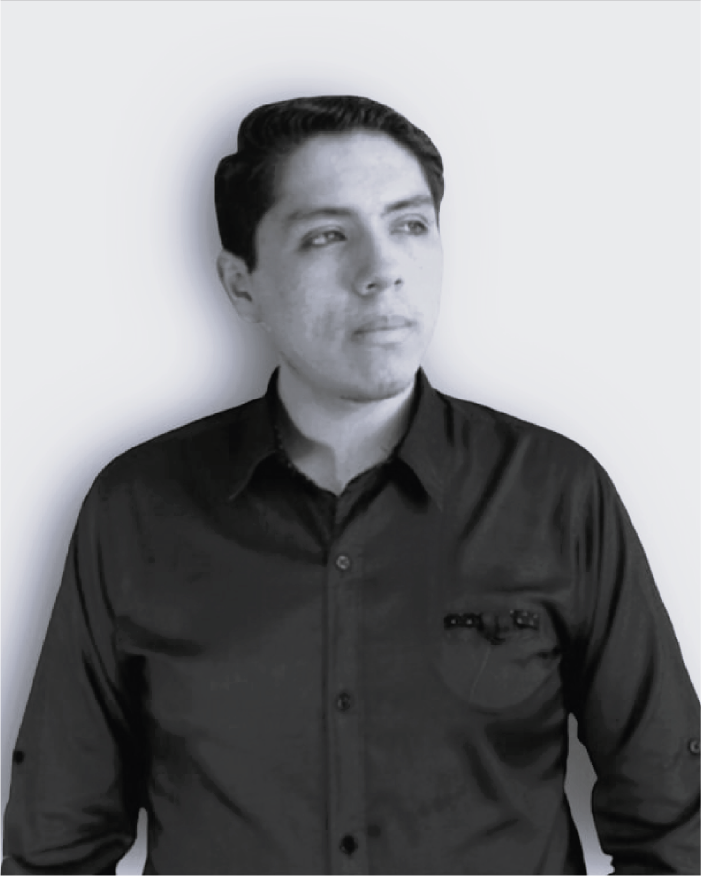
\includegraphics[width=1in,height=1.25in,clip,keepaspectratio]{author2.png}}]{Christopher Antonio Pillihuamán Santiago}
		Es Bachiller en Ingeniería de Sistemas de la Información por la Universidad San Ignacio de Loyola (USIL), Lima, Perú. Cuenta con más de 7 años de experiencia en desarrollo de software y experiencia profesional como Analista Programador, donde ha desarrollado sistemas empresariales utilizando tecnologías como Angular, Spring Boot y MySQL. Ha participado en más de 20 proyectos académicos y profesionales aplicando arquitecturas limpias, metodologías ágiles y principios SOLID. Sus áreas de interés incluyen desarrollo fullstack, aplicaciones móviles, aprendizaje automático aplicado y tecnologías asistivas para poblaciones con necesidades especiales.
	\end{IEEEbiography}
	
	\begin{IEEEbiography}[{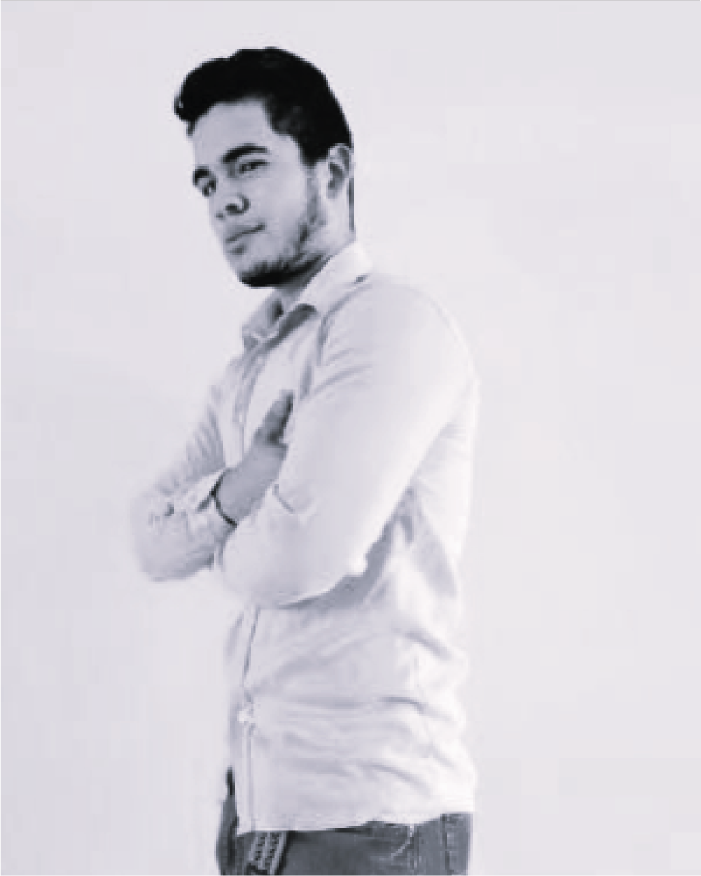
\includegraphics[width=1in,height=1.25in,clip,keepaspectratio]{author3.png}}]{Jhafet Martín Cánepa Maceda}
		Es Bachiller en Ingeniería de Sistemas de la Información por la Universidad San Ignacio de Loyola (USIL), Lima, Perú, con reconocimiento de Matrícula de Honor y Quinto Superior. Actualmente cursa la Maestría en Inteligencia Artificial Generativa en la Universidad de São Paulo, Brasil. Cuenta con más de 2 años de experiencia profesional como Desarrollador de Software en instituciones como la Universidad Nacional de Tumbes, la Universidad Nacional Mayor de San Marcos y el Instituto Nacional de Salud del Niño. Posee publicaciones científicas en revisión internacional sobre reconocimiento de emociones faciales mediante redes neuronales convolucionales y lineamientos de experiencia de usuario para plataformas educativas, además de una patente en trámite ante INDECOPI sobre serious games para reconocimiento de emociones en personas con autismo. Sus áreas de investigación incluyen inteligencia artificial, aprendizaje automático, aplicaciones móviles para salud y tecnologías asistivas.
	\end{IEEEbiography}
	
	\begin{IEEEbiography}[{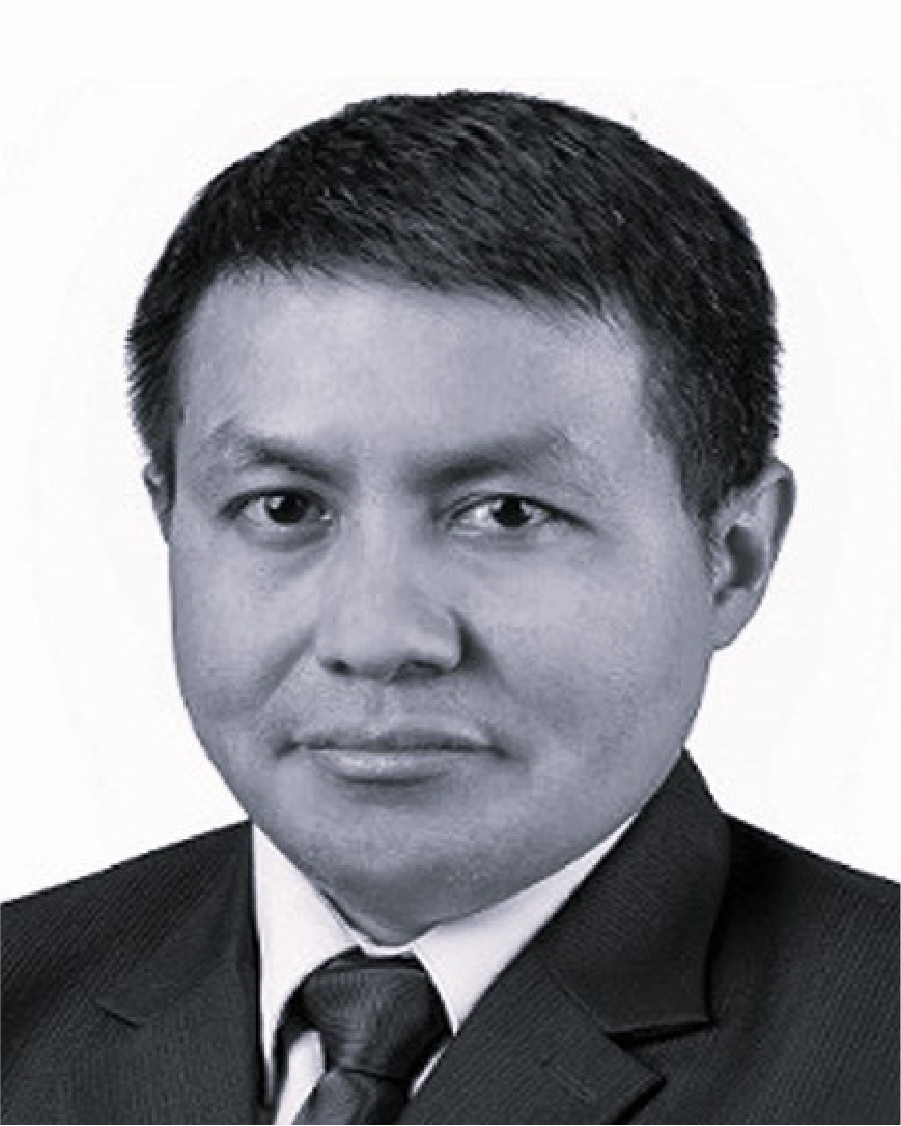
\includegraphics[width=1in,height=1.25in,clip,keepaspectratio]{author4.png}}]{Jomark Pablo Noriega Zapata}
		Es Doctor en Ingeniería de Sistemas e Informática por la Universidad Nacional Mayor de San Marcos (UNMSM), Perú. Cuenta con más de 25 años de experiencia en el diseño, desarrollo y liderazgo de proyectos tecnológicos en el sector financiero, habiendo participado en iniciativas estratégicas en más de doce instituciones financieras. Su trayectoria profesional se ha centrado en la transformación digital, la implementación de soluciones tecnológicas a gran escala y la optimización de procesos de negocio. Sus líneas de investigación incluyen la tecnología financiera (FinTech), el aprendizaje automático aplicado a la predicción del riesgo crediticio, la analítica de datos y la gestión de sistemas de información.
	\end{IEEEbiography}
	
	\begin{IEEEbiography}[{
\includegraphics[width=1in,height=1.25in,clip,keepaspectratio]{author5.png}}]{Juan Orlando Salazar Campos}
		Es egresado del Doctorado en Ingeniería de Sistemas e Informática por la Universidad Nacional Mayor de San Marcos (UNMSM), con Máster en Ciencias de la Computación por la Pontificia Universidad Católica del Perú (PUCP) y Máster en Ingeniería Industrial con mención en Gestión de Operaciones por la Universidad Nacional de Trujillo (UNT). Es Ingeniero Informático colegiado, Investigador RENACYT y miembro Senior de IEEE. Profesional con experiencia en instituciones públicas y privadas como director de programas universitarios, docente, integrante de comités de calidad y acreditación, y líder de proyectos de automatización y desarrollo de aplicaciones. Ha participado en investigaciones como responsable, asesor y colaborador. Se desempeña como Evaluador Senior de Programas de Ingeniería (ICACIT), evaluador SINEACE, evaluador externo de Concytec y ProInnovate.
	\end{IEEEbiography}
	
	\begin{IEEEbiography}[{
\includegraphics[width=1in,height=1.25in,clip,keepaspectratio]{author6.png}}]{Kenny Disney Neira Neira}
		Es Ingeniero de Sistemas con especialización en Gestión de Proyectos y metodologías ágiles, con sólida experiencia en inteligencia artificial y asesoría a startups. Cuenta con amplia trayectoria en el diseño e implementación de prácticas innovadoras orientadas a la creación de PMOs estratégicas, aplicando enfoques como Value Ring y el modelo de madurez OPM3. Se desempeña como docente universitario en instituciones como la Universidad San Ignacio de Loyola (USIL), la Universidad de Ingeniería y Tecnología (UTEC) y la Escuela de Postgrado de la UTP, donde dicta cursos vinculados a sistemas inteligentes, gestión de proyectos, metodologías ágiles e innovación tecnológica. Asimismo, ha liderado y coordinado iniciativas académicas y tecnológicas, mentorando proyectos de fin de carrera y guiando la aplicación de marcos como Scrum, Kanban, DevOps y Lean Startup para la solución de problemáticas reales. Sus áreas de interés incluyen la inteligencia artificial aplicada, la gestión estratégica de proyectos, la transformación digital, el desarrollo de PMOs, la innovación educativa y el análisis de datos.
	\end{IEEEbiography}
	\EOD
\end{document}
